\documentclass[12pt,a4paper]{article}

\usepackage[margin=1in]{geometry}
\usepackage[T1]{fontenc}
\usepackage[utf8]{inputenc}
\usepackage{lmodern}
\usepackage{setspace}
\usepackage{booktabs}
\usepackage{array}
\usepackage{tabularx}
\usepackage{makecell}
\usepackage{graphicx}
\usepackage{float}
\usepackage{hyperref}
\usepackage{enumitem}
\usepackage{xurl}
\usepackage{hanging}

\hypersetup{
    colorlinks=true,
    linkcolor=black,
    urlcolor=blue,
    citecolor=black
}

\setstretch{1.2}
\setlength{\parskip}{0.6em}
\setlength{\parindent}{0pt}
\setlength{\emergencystretch}{2em}

\begin{document}

\begin{titlepage}
\centering
\vspace*{\fill}

{\LARGE \textbf{Stylometric Patterns in Large Language Model Outputs: Comparing Linguistic Signatures of Human and AI-Generated Texts}\par}

\vspace{1.5cm}

{\Large Amir Haziq\par}

\vspace{1cm}

{\large Student ID: 230190311\par}
{\large Word count: 5,474\par}

\vspace*{\fill}
\end{titlepage}

\section*{Structured Abstract}

\textbf{Background:} As the use of Large Language Models (LLMs) grows in educational writing, it is necessary to determine whether machine-generated text can be distinguished from human writing through measurable stylistic features rather than just topic content.

\textbf{Objective:} The goal of this project is to investigate whether stylometric analysis can differentiate academic abstracts written by humans from rewrites of the same source texts produced by LLMs, and whether the same analytical workflow can support multiclass attribution across five classes: one human class and four LLM families.

\textbf{Methods:} A reproducible pipeline controlled by a YAML configuration file was used to generate rewritten abstracts from four LLMs using matched human source abstracts. There were 1,000 texts in the final corpus, 200 of which were human abstracts and 800 of which were produced abstracts. The dataset was analysed using six feature families: lexical, syntactic, combined, writeprints, stylometrix, and stanza-style proxies. Binary classification compared human writing against one model at a time, while multiclass classification compared the human class against the four model classes together using Logistic Regression and Random Forest with grouped cross-validation by \texttt{source\_id}. Supporting semantic overlap was evaluated using ROUGE and a simplified METEOR-style score.

\textbf{Results:} All four binary human-versus-model tasks produced above-chance discrimination, with the strongest result obtained for Gemma using combined features and Random Forest (mean accuracy = 0.8400, mean F1 = 0.8385, mean ROC-AUC = 0.9249), and similarly strong performance for Llama using combined features and Random Forest (a mean F1 = 0.8252). In the multiclass setting, the strongest configuration was combined Random Forest, which achieved a mean accuracy of 0.5390, mean macro-F1 of 0.5378, and a mean ROC-AUC of 0.8209 across the five classes. Across both tasks, combined and syntactic feature sets consistently outperformed lexical-only and weaker proxy feature families, suggesting that structural cues were more informative than vocabulary-summary measures alone. Semantic-overlap scores showed that generated texts remained substantially aligned with their source abstracts, with Mistral producing the highest overlap values (ROUGE-1 F1 = 0.7346; METEOR = 0.6879).

\textbf{Conclusion:} The findings provide evidence that human-written and LLM-generated academic abstracts can be distinguished with meaningful, though not perfect, reliability in this source-matched setting, particularly when structural feature sets are used. The project therefore supports a cautious claim of stylistic discrimination rather than absolute separability. However, the study remains a pilot, and the results should be interpreted carefully because they are limited by prompt choice, domain specificity, and the use of proxy feature families.

\clearpage
\tableofcontents

\newpage

\section{Introduction}

\subsection{Background}

In a world where artificial intelligence and machine learning are rapidly expanding, Large Language Models (LLMs) have become a powerful tool in natural language generation, producing contextual text and images on a huge scale. Education, research, and even everyday communication are increasingly integrated through the use of these systems. This creates a practical and scholarly problem. In educational contexts, people are now increasingly driven to produce generated text for their papers and assessments. There is evidence showing that ChatGPT is widely used in academic research, particularly for drafting essays, summarising papers, and generating comments and reviews (Huang \& Tan, 2023; Geng \& Trotta, 2024). Even though it is becoming increasingly common, trained LLMs generate vast amounts of creative text that appears human-like, and previous research has suggested that humans often struggle to distinguish between human writing and AI-generated content (Zaitsu et al., 2025). It is no longer sufficient to ask whether generated text is factually plausible or readable. Even so, this machine-generated writing surely leaves stylistic traces when the same source material is used as a constraint in the generated text.

Stylometry was introduced in the 20th century as the study of writing style for tasks such as identifying authors, comparing disputed texts, and examining stylistic variation across writers. Stylometric analysis highlights quantitative linguistic and structural indicators that identify variation and authorship through features of style (L\'opez-Escobedo et al., 2013). Although LLMs have proven extremely useful at replicating superficial stylistic features, it remains challenging to capture subtler qualities of human writing, especially innovation, profound causal reasoning, and genuine authorial voice (Mikros, 2025).

This project studies academic abstracts because they are compact, structured, and information-dense. Systematic differences between LLM-generated and human-written abstracts could affect authorship analysis, educational integrity, and human-AI writing research. Since LLM stylometric patterns remain insufficiently explored, this study examines whether human and generated abstracts show distinguishable patterns across lexical diversity, sentence structure, and sentiment polarity (Przystalski et al., 2025).

These trends matter for debates about AI originality and authenticity, but reliability should not be overstated. AI-output detectors can still miscalculate or overfit, raising issues of trust and precision (Erol et al., 2025). Academic writing is also highly constrained, which may reduce the stylistic variance on which stylometry depends. Therefore, the report describes outputs cautiously, justifies feature design, and interprets results in relation to technical and methodological limitations.

\subsection{Aims and Objectives}

This report presents a config-driven comparison of human and LLM-generated academic abstracts. The pipeline generates outputs from multiple LLMs, extracts stylometric feature families, and evaluates binary and multiclass classification. The main purpose is to test whether selected linguistic features can distinguish human writing from different LLM outputs.

The report objectives are stated as follows:

\begin{itemize}
    \item Collect contextual samples of text of academic papers from open data sources such as arXiv or Semantic Scholar.
    \item Collect generated-text datasets from multiple LLMs (Llama 3.1, Gemma 2, Qwen 2.5, and Mistral 7B) using a factual prompt.
    \item Evaluate semantic overlap between LLM-generated and human-written abstracts using ROUGE and METEOR-style metrics.
    \item Extract a range of stylometric features using NLP techniques (lexical, syntactic complexity and sentiment analysis)
    \item Evaluate these features for their reliability in classifying text origin.
    \item Develop a visual representation demonstrating the stylistic difference between LLMs and humans interactively.
\end{itemize}

\section{Literature Review}

\subsection{Stylometry as a Field}

Stylometry provides the methodological starting point for this project because it treats writing style as something that can be measured rather than only described impressionistically. Stylometry is introduced as a quantitative approach to authorship, where features such as word use, sentence form, and other recurrent linguistic habits can help distinguish one writer from another (Holmes \& Kardos, 2003). This foundation matters because the present project also assumes that style leaves measurable traces, but it applies that assumption to a newer authorship problem: whether human-written academic abstracts can be separated from LLM-generated rewrites.

The field has developed well beyond early manual comparison. Stylometry covers authorship attribution, authorship verification, author profiling, and adversarial stylometry, and these tasks commonly rely on computational feature extraction and supervised classification (Neal et al., 2018). Zheng et al. (2006) similarly demonstrate the value of using multiple writing-style feature groups, including lexical, syntactic, structural, and content-specific features, for identifying authorship in online messages. These studies support the general validity of feature-based authorship analysis and justify treating stylometry as a credible methodological tradition rather than as an experimental novelty.

However, traditional stylometry also has an important limitation for this study. Most of its established applications were designed for human-to-human comparison, where the task is to decide which person wrote a text or whether two texts share a human author. Koppel et al. (2009) note that real authorship attribution is already difficult when the candidate set is large, when training data are limited, or when the task does not fit a simple closed-set design. Human-versus-machine attribution adds a further complication because the ``author'' may not have a stable personal style in the human sense. An LLM output is shaped by pretraining data, decoding settings, prompt design, and the source text being rewritten. Therefore, the literature supports the use of stylometry, but it also warns against assuming that methods validated for human authors automatically transfer to generated text without careful evaluation.

\subsection{LLM-Generated Text and Detection}

The growth of LLM-generated writing has created a new detection problem. Earlier discussion of language-model release risks already recognised that generated text could be socially useful while also creating risks around misuse, authenticity, and attribution (Solaiman et al., 2019). More recent detection research has attempted to respond to this problem through automatic classifiers, watermarking ideas, probability-based methods, and human evaluation. Mitchell et al. (2023), for example, propose DetectGPT, a zero-shot method based on the observation that model-generated text can occupy distinctive regions of a language model's probability function. This line of work is important because it shows that generated text may be detectable without relying only on visible surface errors.

Dhaini, Poelman, and Erdogan (2023) provide a useful survey of ChatGPT-generated text detection and show why the problem remains difficult. Their review highlights that LLM outputs are fluent enough to make simple human judgement unreliable, while automatic detectors can be sensitive to training data, genre, prompt conditions, and the model being tested. This is directly relevant to academic writing, where generated abstracts may follow the same formal conventions as human abstracts and may not contain obvious grammatical or factual errors.

At the same time, the detection literature has limitations that motivate this project. Much existing work is model-specific, often concentrating on ChatGPT or on a single generator, which makes it difficult to know whether the observed signal is a general human-versus-machine distinction or only the signature of one model family. Detection studies also often rely on content-based signals, token probabilities, or broad textual classifiers rather than explicitly stylometric feature families. This can make the result less interpretable as evidence of style. A further weakness is that generated and human texts are not always source-matched. If human texts and machine texts discuss different topics, a classifier may learn subject matter rather than authorship origin. For this reason, source-matched corpora are especially important: they reduce topic confounding by comparing human abstracts with generated rewrites of the same source material.

\subsection{Feature Design in Stylometric Classification}

Feature design is central to stylometric classification because the features define what the classifier is allowed to treat as evidence. Lexical features such as type-token ratio, average word length, hapax ratio, and vocabulary-frequency measures are useful because they are simple, interpretable, and historically common in authorship attribution. However, lexical evidence is also vulnerable to topic contamination. If two groups of texts discuss different subject matter, vocabulary differences may reflect domain content rather than writing style. This risk is reduced but not removed in a source-matched design, since LLM rewrites can still preserve many of the same content words from the original abstract.

Syntactic and structural features offer a stronger theoretical basis for this project because they capture how information is organised rather than only which content words appear. Sentence length, punctuation behaviour, part-of-speech patterns, function-word distribution, and measures of syntactic complexity are less directly tied to the research topic of the abstract. They are therefore more likely to represent stylistic regularities in how humans and models arrange claims, methods, results, and conclusions. This does not mean that syntactic features are perfectly topic-free, but it makes them methodologically preferable when the goal is to detect stylistic signal under controlled content conditions.

The importance of comparing feature families is supported by recent work on human and LLM-generated text. Przystalski et al. (2025) show that stylometric methods can recognise human and LLM-generated texts even in short samples, which is especially relevant for abstracts because they provide limited text per document. Their work is important not simply because it reports successful classification, but because it supports the idea that multiple stylistic feature groups should be evaluated rather than assuming that one feature type is sufficient. Zaitsu et al. (2025) also show that stylometry can reveal AI authorship while humans struggle to make the same distinction unaided. Together, these findings justify the present study's use of several feature families, including lexical, syntactic, combined, writeprints-style, stylometrix-style, and stanza-style proxy features.

This feature-family approach also shapes the choice of classifiers. Logistic Regression is useful as an interpretable linear baseline because it tests whether the feature spaces contain separable signal without requiring a highly complex model. Random Forest provides a complementary non-linear comparison because it can capture feature interactions and threshold effects. This choice is also consistent with comparative authorship-attribution research, where machine learning methods are commonly evaluated as competing approaches for identifying stylistic signals in text (Jockers \& Witten, 2010). However, the classifier cannot compensate for weak corpus design. When each human abstract is paired with several generated rewrites, random splitting can leak source-linked information across training and test folds. Group-aware validation is therefore needed so that evaluation reflects stylometric discrimination rather than memorisation of source-specific content.

\subsection{Gap Filled by This Study}

The literature therefore supports four connected conclusions. First, stylometry is a well-established methodology for measuring writing style and has a strong track record in human authorship analysis. Second, LLM-generated text creates a related but different attribution problem because machine outputs are shaped by model architecture, prompting, and decoding rather than by a stable human authorial identity. Third, current AI-text detection research is often model-specific, content-dependent, or focused on broad detector performance rather than interpretable stylometric feature comparison. Fourth, feature design matters because lexical features alone can be contaminated by topic, while syntactic and structural evidence may provide more robust stylistic signals.

This study addresses that gap by testing multiple LLM families against source-matched human academic abstracts using a multi-feature stylometric pipeline. Instead of asking only whether one detector can identify one model's outputs, it compares human writing with outputs from Llama, Gemma, Qwen, and Mistral under the same source constraints. It also evaluates several feature families and uses group-aware validation by \texttt{source\_id} to reduce leakage from paired abstracts. The project therefore contributes a controlled pilot study of human-versus-LLM stylometry in academic abstracts, with emphasis on feature-family comparison, source matching, and cautious interpretation rather than absolute detection claims.

\subsection{The Research Questions}

The project structure is guided by the following research questions:

\begin{itemize}
    \item Can we distinguish human-written academic abstracts from LLM-generated with feature-based stylometry through rewriting the same source papers?
    \item Which feature families contribute most strongly to the linguistic discrimination in both binary classification and the five-class multiclass setting: human, Llama, Gemma, Qwen, and Mistral?
    \item To what extent can the current outputs support multiclass attribution of academic abstracts across human and multiple LLM sources?
\end{itemize}

These research questions are justified by the gap identified in the literature. The first question is necessary because the project aims to test stylistic separability in a controlled source-matched setting rather than relying on topic differences between unrelated texts. The second question is important because stylometric performance depends heavily on feature design, so the report must determine which types of linguistic evidence are most informative not only in binary tasks but also in the full five-class multiclass setting. The third question is included because distinguishing human writing from one model is a simpler task than separating several LLM families at once, and this helps to evaluate how far the current pilot outputs support broader attribution claims. Together, these questions move from basic human-versus-LLM separation to the more specific issue of which stylistic signals matter most and how far the present evidence can be interpreted.

\section{Methods Plan}

\subsection{Data Collection Procedure}

The project used a supervised stylometric classification design. Human-written academic abstracts were collected through the Scopus library using the search key `machine learning' with a computer science field filter, and this dataset acted as one class, while LLM-generated abstract rewrites with the matched source abstract were treated as comparison classes. This overall design ensures that both binary (human versus one model) and multiclass classification (human plus several model labels simultaneously) can be executed in this research.

The human data source contains Scopus-derived abstracts which includes \texttt{source\_id}, \texttt{title}, \texttt{abstract}, \texttt{year}, and \texttt{doi}. The topic of machine learning was chosen because it provides a large and current body of academic abstracts within one coherent research area. Restricting the corpus to one topic helps reduce unnecessary variation in subject matter, so that later differences are more likely to reflect writing style rather than major topic differences between papers. The abstracts are processed using \texttt{source\_id} as the grouping key while working on the main text field (abstracts).

Each sample from the human text is inserted into different prominent models to generate text while consistently remaining in the format of a human abstract. The main purpose of this is to preserve the context and similarity of the original human research text. The analysed `master\_with\_features.csv' provides a balanced subset of 1000 texts: 200 human abstracts and 800 generated texts, with 200 for each different LLM.

In the LLM abstract dataset, each of the four models contains 200 generated abstracts through the following models:

\begin{itemize}
    \item Llama -3.1-8b-instruct
    \item Gemma-2-9b-it
    \item Qwen-2.5-7b-instruct
    \item Mistral-7b-instruct-v0.3
\end{itemize}

These four models were chosen because they represent different widely used open-weight instruction-tuned LLM families that were feasible to run within the project scope. Using several model families rather than only one makes the comparison more meaningful, because it allows the study to test whether any stylometric patterns are specific to one generator or whether similar distinctions can still be observed across multiple LLM sources. Furthermore, these models are open-sourced and can be used publicly by other researchers.

The generation pipeline uses the original human abstract as the source text, and the LLM rewrites it into a new LLM-generated abstract through one factual prompt style. All saved rows are labelled with the factual prompt type configuration:

\begin{quote}
``You are an academic writer in computer science.

Task:
Produce one original abstract in English (220--300 words) for a machine learning study, based on the source abstract.

Requirements:
\begin{enumerate}[label=\arabic*., leftmargin=2em]
    \item Preserve the same research context, thematic focus, and academic tone.
    \item Follow a standard abstract flow: background $\rightarrow$ objective $\rightarrow$ method $\rightarrow$ results $\rightarrow$ conclusion.
    \item Keep the writing factual, objective, and evidence-oriented.
    \item Do not copy sentences or long phrases from the source.
    \item Do not add citations, references, headings, or bullet points.
    \item Return only the rewritten abstract text.
\end{enumerate}
'' 
\end{quote}

This prompt was chosen because it keeps the generation task controlled while still allowing the models to produce their own wording and structure. It constrains the output length, academic tone, and abstract organisation so that the generated texts remain comparable to the human source abstracts. At the same time, the instruction not to copy long phrases helps prevent near-duplicate outputs, making the later stylometric comparison more meaningful as an analysis of rewriting style rather than simple textual overlap.

The data collection is stored in JSON format with metadata including the model and prompt type. In this case, the author name is excluded to prevent any breach of personal data, ensuring that the project is performed under ethical consideration. Even so, the collection of data starts only after ethical approval.

A deductive approach is applied using predefined hypotheses that measure differences in stylistic structural patterns for group classification (LLMs or humans). A quantitative approach was selected because the project aims to test whether measurable stylistic differences can be identified consistently across many texts, rather than relying on subjective reading or impression-based judgement. ROUGE (Recall-Oriented Understudy for Gisting Evaluation) is used as a supporting semantic-overlap measure because it compares the overlap of units such as words, short phrases, and longest matching sequences between two texts. In this project, it is used to check whether the LLM-generated abstracts remain close in content to their human source abstracts. ROUGE was chosen because it is efficient for automatic evaluation (Lin, 2004), straightforward to apply to source-and-rewrite pairs, and useful as a simple validity check that the generated texts are not drifting too far from the original research content. METEOR was also selected as a supporting metric because it compares unigram precision and recall while considering word-order similarity, making it useful for checking whether rewrites remain close to the source even when wording changes (Banerjee and Lavie, 2005).

\subsection{Analysis Methods}

Six feature sets are compared in the analysis. The \texttt{lexical} feature set contains word-count and vocabulary-summary measures such as total word count, number of types, average word length, type-token ratio, and hapax ratio. The \texttt{syntactic} feature set contains structural and distributional features such as sentence count, average and standard deviation of sentence length, punctuation rates, function-word frequencies, hedge markers, and citation markers. The \texttt{combined} feature set merges the lexical and syntactic sets so that both vocabulary-level and structural evidence are available to the classifier.

The remaining three sets are proxy feature families intended to widen the stylistic comparison. The \texttt{writeprints} set is a lightweight writeprints-style proxy including character-per-word ratio, uppercase ratio, digit ratio, punctuation ratio, and frequent character trigram features. The \texttt{stylometrix} set is a lightweight stylometrix-style proxy including rates of long words, modal verbs, and pronouns. The \texttt{stanza} set is a lightweight stanza-style proxy based on simple surface distributions, including rates of words ending in \texttt{-ing}, \texttt{-ed}, \texttt{-ly}, and nominalising endings such as \texttt{-tion} and \texttt{-sion}. These three proxy sets are not full reproductions of the original external toolkits, so they should be interpreted as approximations rather than direct implementations.

\begin{table}[H]
\centering
\small
\begin{tabularx}{\textwidth}{>{\raggedright\arraybackslash}p{2.7cm} X}
\toprule
Feature set & Exact contents \\
\midrule
\texttt{lexical} & \texttt{word\_count}, \texttt{type\_count}, \texttt{avg\_word\_len}, \texttt{type\_token\_ratio}, \texttt{hapax\_ratio}. \\
\texttt{syntactic} & \texttt{sentence\_count}, \texttt{avg\_sentence\_len\_words}, \texttt{std\_sentence\_len\_words}; punctuation-rate features for comma, semicolon, colon, hyphen, question mark, exclamation mark, left bracket, right bracket, and quotation mark; function-word frequency features for \texttt{the}, \texttt{a}, \texttt{an}, \texttt{and}, \texttt{or}, \texttt{but}, \texttt{if}, \texttt{while}, \texttt{because}, \texttt{as}, \texttt{of}, \texttt{in}, \texttt{on}, \texttt{for}, \texttt{to}, \texttt{from}, \texttt{by}, \texttt{with}, \texttt{without}, \texttt{about}, \texttt{at}, \texttt{into}, \texttt{through}, \texttt{between}, \texttt{among}, \texttt{is}, \texttt{are}, \texttt{was}, \texttt{were}, \texttt{be}, \texttt{been}, \texttt{being}, \texttt{that}, \texttt{this}, \texttt{these}, \texttt{those}, \texttt{it}, \texttt{its}, \texttt{their}, \texttt{there}, \texttt{which}, \texttt{who}, \texttt{whom}, \texttt{whose}, \texttt{not}, \texttt{no}, \texttt{can}, \texttt{could}, \texttt{may}, \texttt{might}, \texttt{must}, \texttt{should}, and \texttt{would}; plus \texttt{hedge\_per100w}, \texttt{citation\_year\_per100w}, and \texttt{et\_al\_per100w}. \\
\texttt{combined} & All features from the \texttt{lexical} and \texttt{syntactic} sets combined. \\
\texttt{writeprints} & \texttt{wp\_char\_per\_word}, \texttt{wp\_upper\_ratio}, \texttt{wp\_digit\_ratio}, \texttt{wp\_punct\_ratio}, and \texttt{wp\_top\_tri\_1\_freq} to \texttt{wp\_top\_tri\_10\_freq}, representing the frequencies of the ten most common character trigrams within each text. \\
\texttt{stylometrix} & \texttt{sm\_long\_words\_per100w}, \texttt{sm\_modal\_per100w}, \texttt{sm\_pronoun\_per100w}. \\
\texttt{stanza} & \texttt{st\_ing\_per100w}, \texttt{st\_ed\_per100w}, \texttt{st\_adv\_per100w}, \texttt{st\_nominal\_per100w}. \\
\bottomrule
\end{tabularx}
\caption{Exact feature contents for each configured feature set used in the analysis.}
\label{tab:feature-set-inventory}
\end{table}

Feature extraction is then carried out, followed by classification with \texttt{StratifiedGroupKFold}, using \texttt{source\_id} as the grouping variable. This approach is appropriate because the design allows each source paper to generate multiple related texts. Group-aware splitting reduces leakage between training and test folds and therefore provides more credible estimates than naive random splitting.

Two classifiers were used: Logistic Regression with standardisation and Random Forest with class balancing. Logistic Regression was chosen as a strong linear baseline because it is widely used in stylometric classification, performs well on structured feature tables, and helps to test whether the feature sets contain linearly separable signal. Random Forest was chosen as a complementary non-linear model because it can capture feature interactions and threshold effects that a linear classifier may miss. Using both models therefore allowed the analysis to compare a simpler interpretable baseline with a more flexible classifier. The configured number of folds was 5, and the random seed was 42. Binary evaluation used accuracy, precision, recall, F1-score, ROC-AUC, Matthews correlation coefficient, and macro-F1. Multiclass evaluation used the same grouped cross-validation logic and reported macro-averaged metrics across all five classes.

\subsection{Digital Artefact Construction}

The digital artefact in this project is the analytical workflow that transforms a collection of human abstracts and model-generated rewrites into measurable evidence about stylistic difference. Its main function is to take paired text data, extract multiple stylometric feature families, evaluate classification performance under leakage-aware cross-validation, and produce saved outputs that can be inspected systematically. In practical terms, the artefact allows the study to move beyond impression-based judgements by generating comparable quantitative evidence for binary human-versus-model classification, five-class multiclass attribution, and semantic-overlap checking.

The artefact also supports interpretation and communication of the findings. It produces feature tables, fold-level evaluation results, summary metrics, and visualisations that show how performance changes across feature families and models. This is important because the research question is not only whether classification is possible, but also which kinds of stylistic evidence contribute most strongly and how consistent those patterns are across the evaluated models. The artefact therefore functions as both an analysis mechanism and a reporting aid, making the results more transparent, inspectable, and easier to compare across experiments.

The project repository is available on GitHub at \url{https://github.com/Haziqmazhar/stylometry_analysis}. This repository contains the source code, configuration file, prompt file, result-generation scripts, and report-related outputs used to construct and document the digital artefact.

\subsection{Ethical Issues}

The flow of the project demonstrates the use of open-source published academic abstracts and generated abstracts derived from the rewriting process of those abstracts. No personal or sensitive personal data were collected, implying a low risk of breaching data privacy. The data are open-source, and the extracted data exclude personal identifiers such as paper authorship (secondary data), while LLM-generated texts are synthetic, raising no privacy concerns. For intellectual property and copyright, the data are obtained from an open website (Scopus) under a Netherlands-based publishing company with a licence, and the generated texts are classified and labelled as AI-produced for responsible use. This project identifies its focal point as linguistic features rather than content and meaning, thereby avoiding bias in relation to sensitive topics. Careful data curation and model adjustment are applied to reduce bias in LLM-generated data. Finally, the outcome of this research should not present stylometric classification as a definitive mechanism for accusing individual authors of misconduct. The results are solely for research purposes concerning stylistic separability in a controlled dataset.

\section{Analysis}

\subsection{Available Evidence and Corpus Balance}

The current local result set contains a balanced five-class corpus and a complete comparative result set for the configured feature families. The master feature table contains 1,000 rows in total: 200 human abstracts, 200 Llama 3.1 abstracts, 200 Gemma 2 abstracts, 200 Qwen 2.5 abstracts, and 200 Mistral 7B abstracts. The result directory contains binary fold files for all four models across all six configured feature families, and multiclass fold files for \texttt{lexical}, \texttt{syntactic}, \texttt{combined}, \texttt{writeprints}, \texttt{stylometrix}, and \texttt{stanza}.

\begin{figure}[H]
\centering
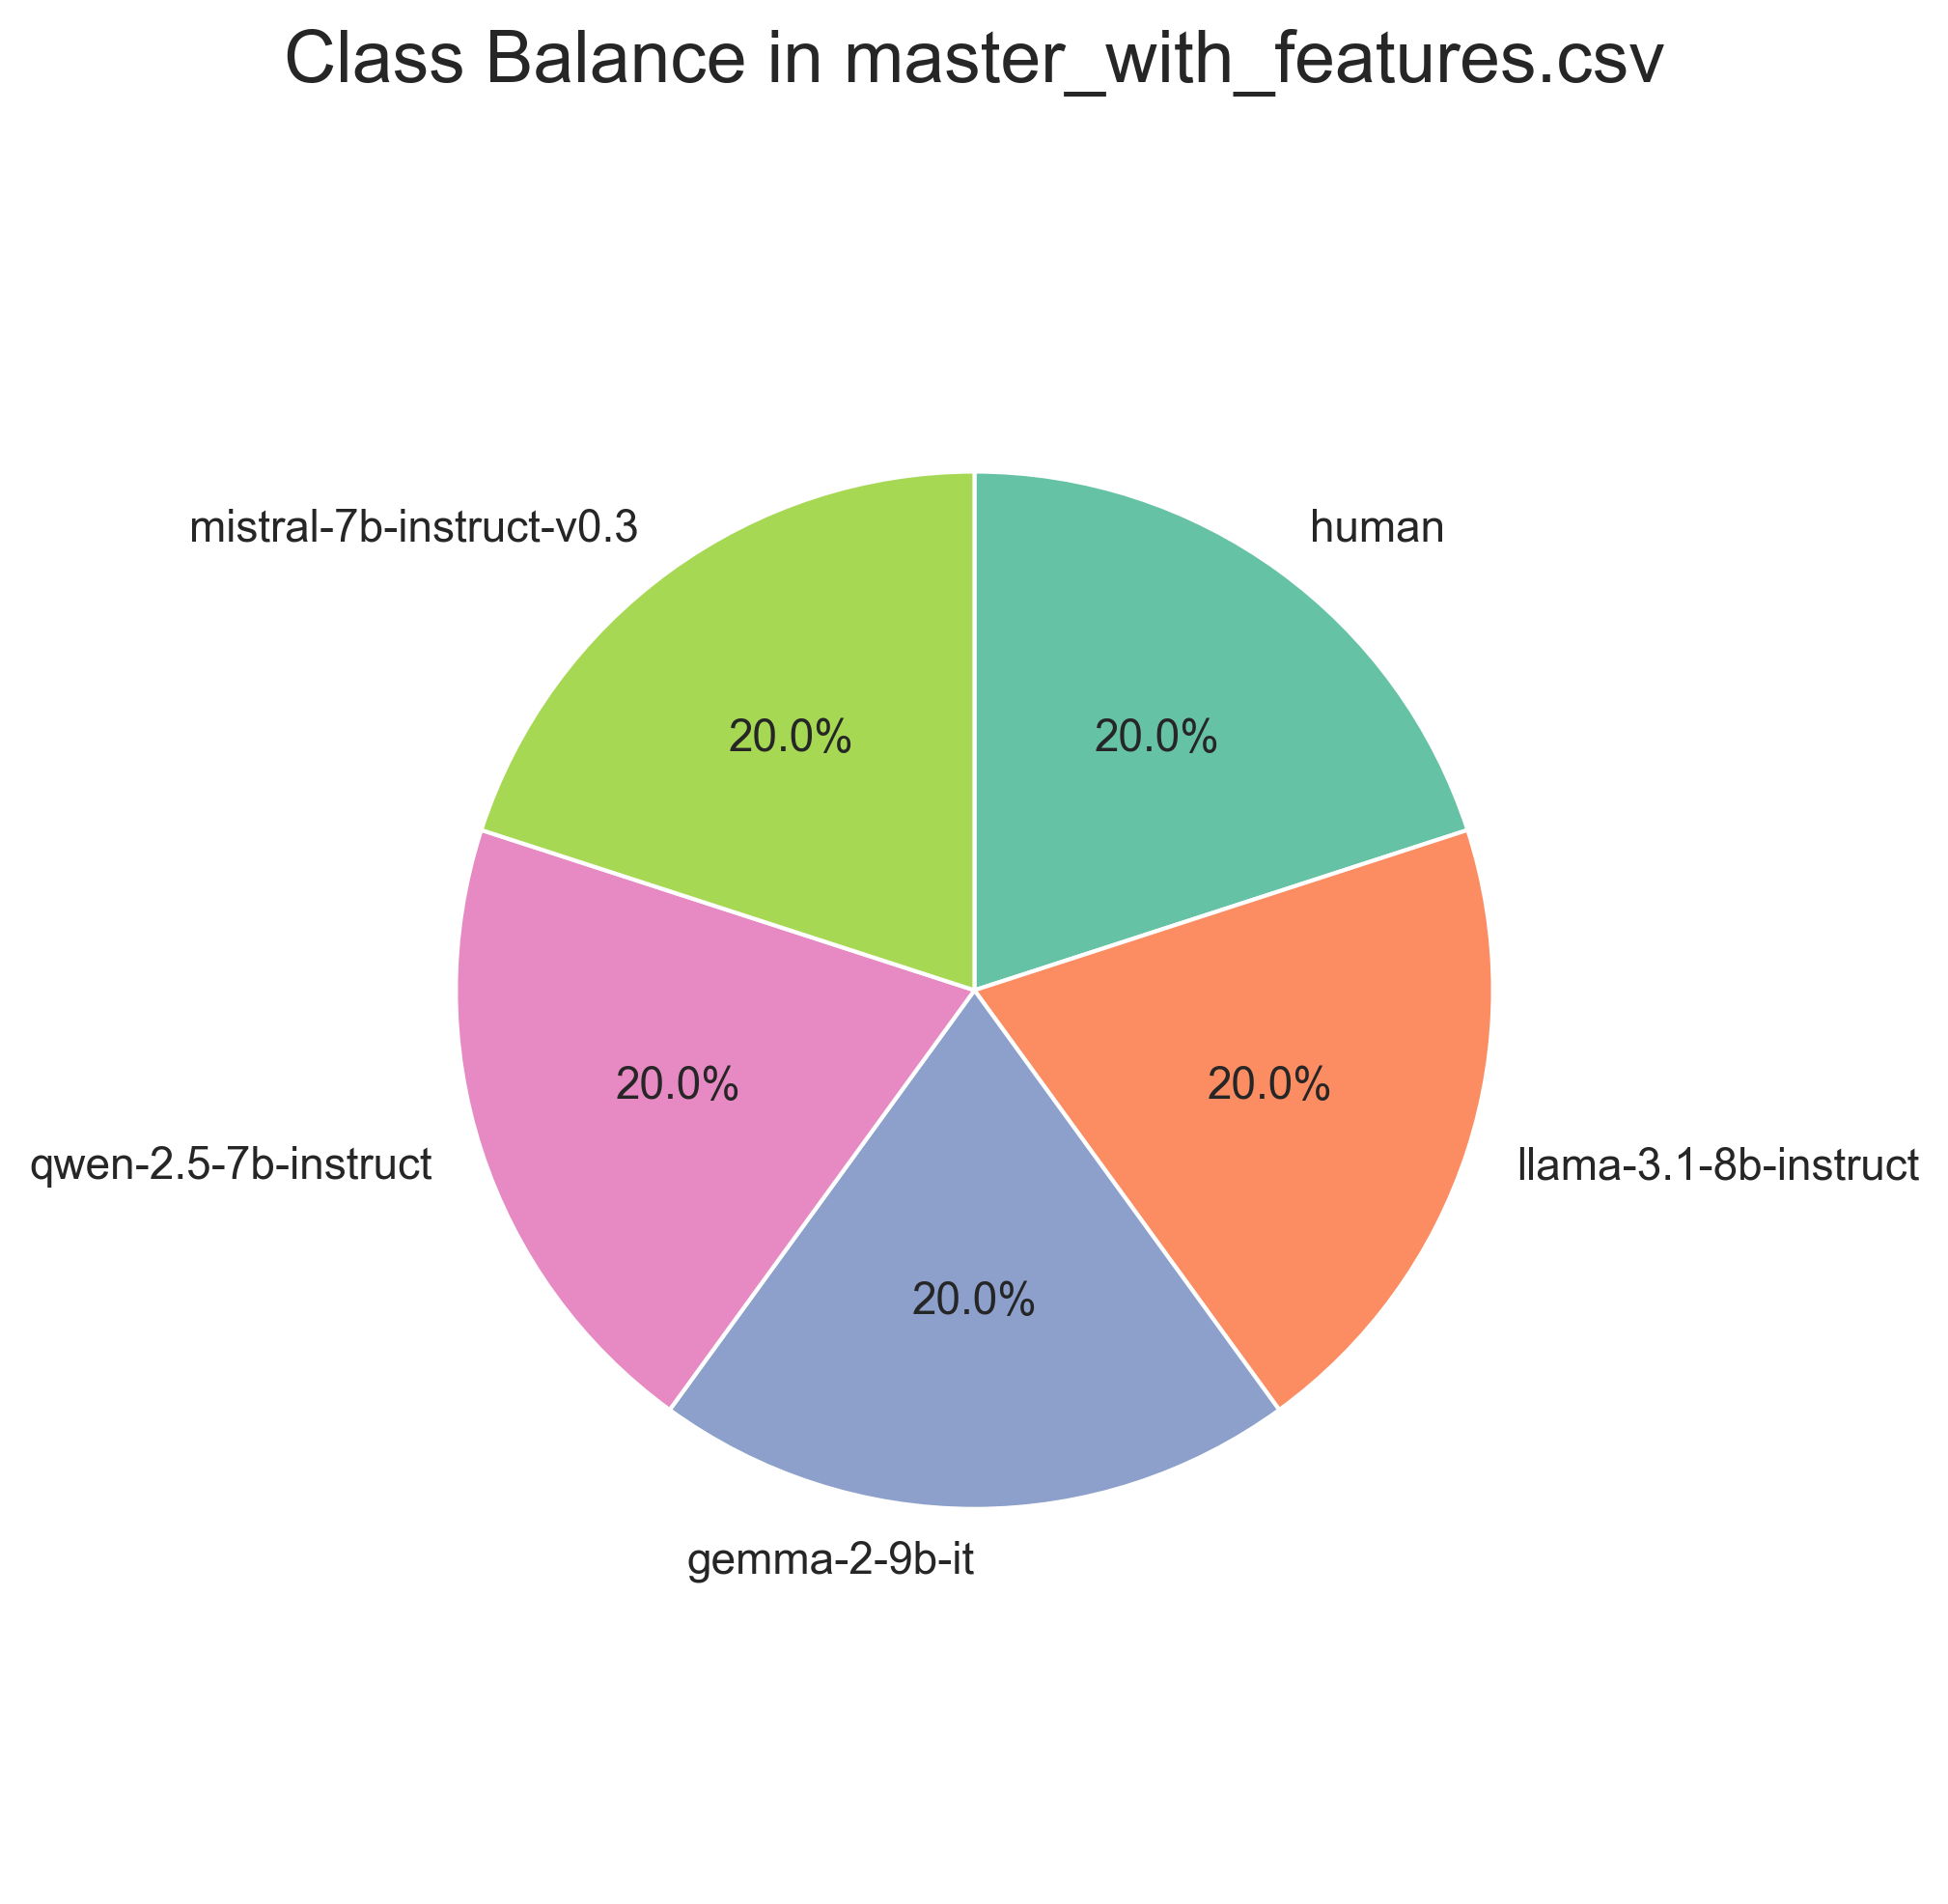
\includegraphics[width=0.7\textwidth]{results/v2/figures/class_balance.png}
\caption{Class balance in \texttt{master\_with\_features.csv}. The analysed pilot subset is balanced across the human class and the four LLM classes represented in the feature table.}
\label{fig:class-balance}
\end{figure}

\subsection{Binary Human-versus-Model Performance Across Feature Families}

The updated binary results show a clear pattern across models. Combined and syntactic feature sets dominate the strongest binary configurations, while the lexical, stanza, writeprints, and stylometrix feature sets are generally weaker. Here, \texttt{stanza}, \texttt{writeprints}, and \texttt{stylometrix} refer to the three proxy feature families described in the methods section. Table~\ref{tab:binary-best} summarises the best binary configuration for each model according to mean F1-score.

\begin{table}[H]
\centering
\small
\begin{tabularx}{\textwidth}{>{\raggedright\arraybackslash}p{4.0cm} >{\raggedright\arraybackslash}p{2.5cm} >{\raggedright\arraybackslash}p{2.8cm} *{4}{>{\centering\arraybackslash}p{1.2cm}}}
\toprule
Target model & Feature set & Estimator & Accuracy & F1 & ROC-AUC & MCC \\
\midrule
\texttt{gemma-2-9b-it} & Syntactic & Logistic Regression & 0.8275 & 0.8276 & 0.9025 & 0.6581 \\
\makecell[l]{\texttt{llama-3.1-8b-}\\\texttt{instruct}} & Combined & Random Forest & 0.8150 & 0.8115 & 0.9075 & 0.6323 \\
\makecell[l]{\texttt{qwen-2.5-7b-}\\\texttt{instruct}} & Combined & Random Forest & 0.7700 & 0.7584 & 0.8573 & 0.5429 \\
\makecell[l]{\texttt{mistral-7b-}\\\texttt{instruct-v0.3}} & Combined & Random Forest & 0.7650 & 0.7621 & 0.8436 & 0.5327 \\
\bottomrule
\end{tabularx}
\caption{Best saved binary configuration for each LLM model, ranked by mean F1-score.}
\label{tab:binary-best}
\end{table}

The best binary result overall is obtained on the Gemma task with syntactic features and Logistic Regression, producing mean accuracy of 0.8275, mean F1 of 0.8276, and mean MCC of 0.6581. The highest binary ROC-AUC is obtained on the Gemma task with combined features and Random Forest, at 0.9338. For Llama 3.1, Qwen 2.5, and Mistral 7B, combined-feature Random Forest is the strongest saved binary configuration. This indicates that not all LLM families are equally separable from the human class under the current feature design, with Gemma appearing easiest to distinguish and Mistral and Qwen proving harder.

\begin{figure}[H]
\centering
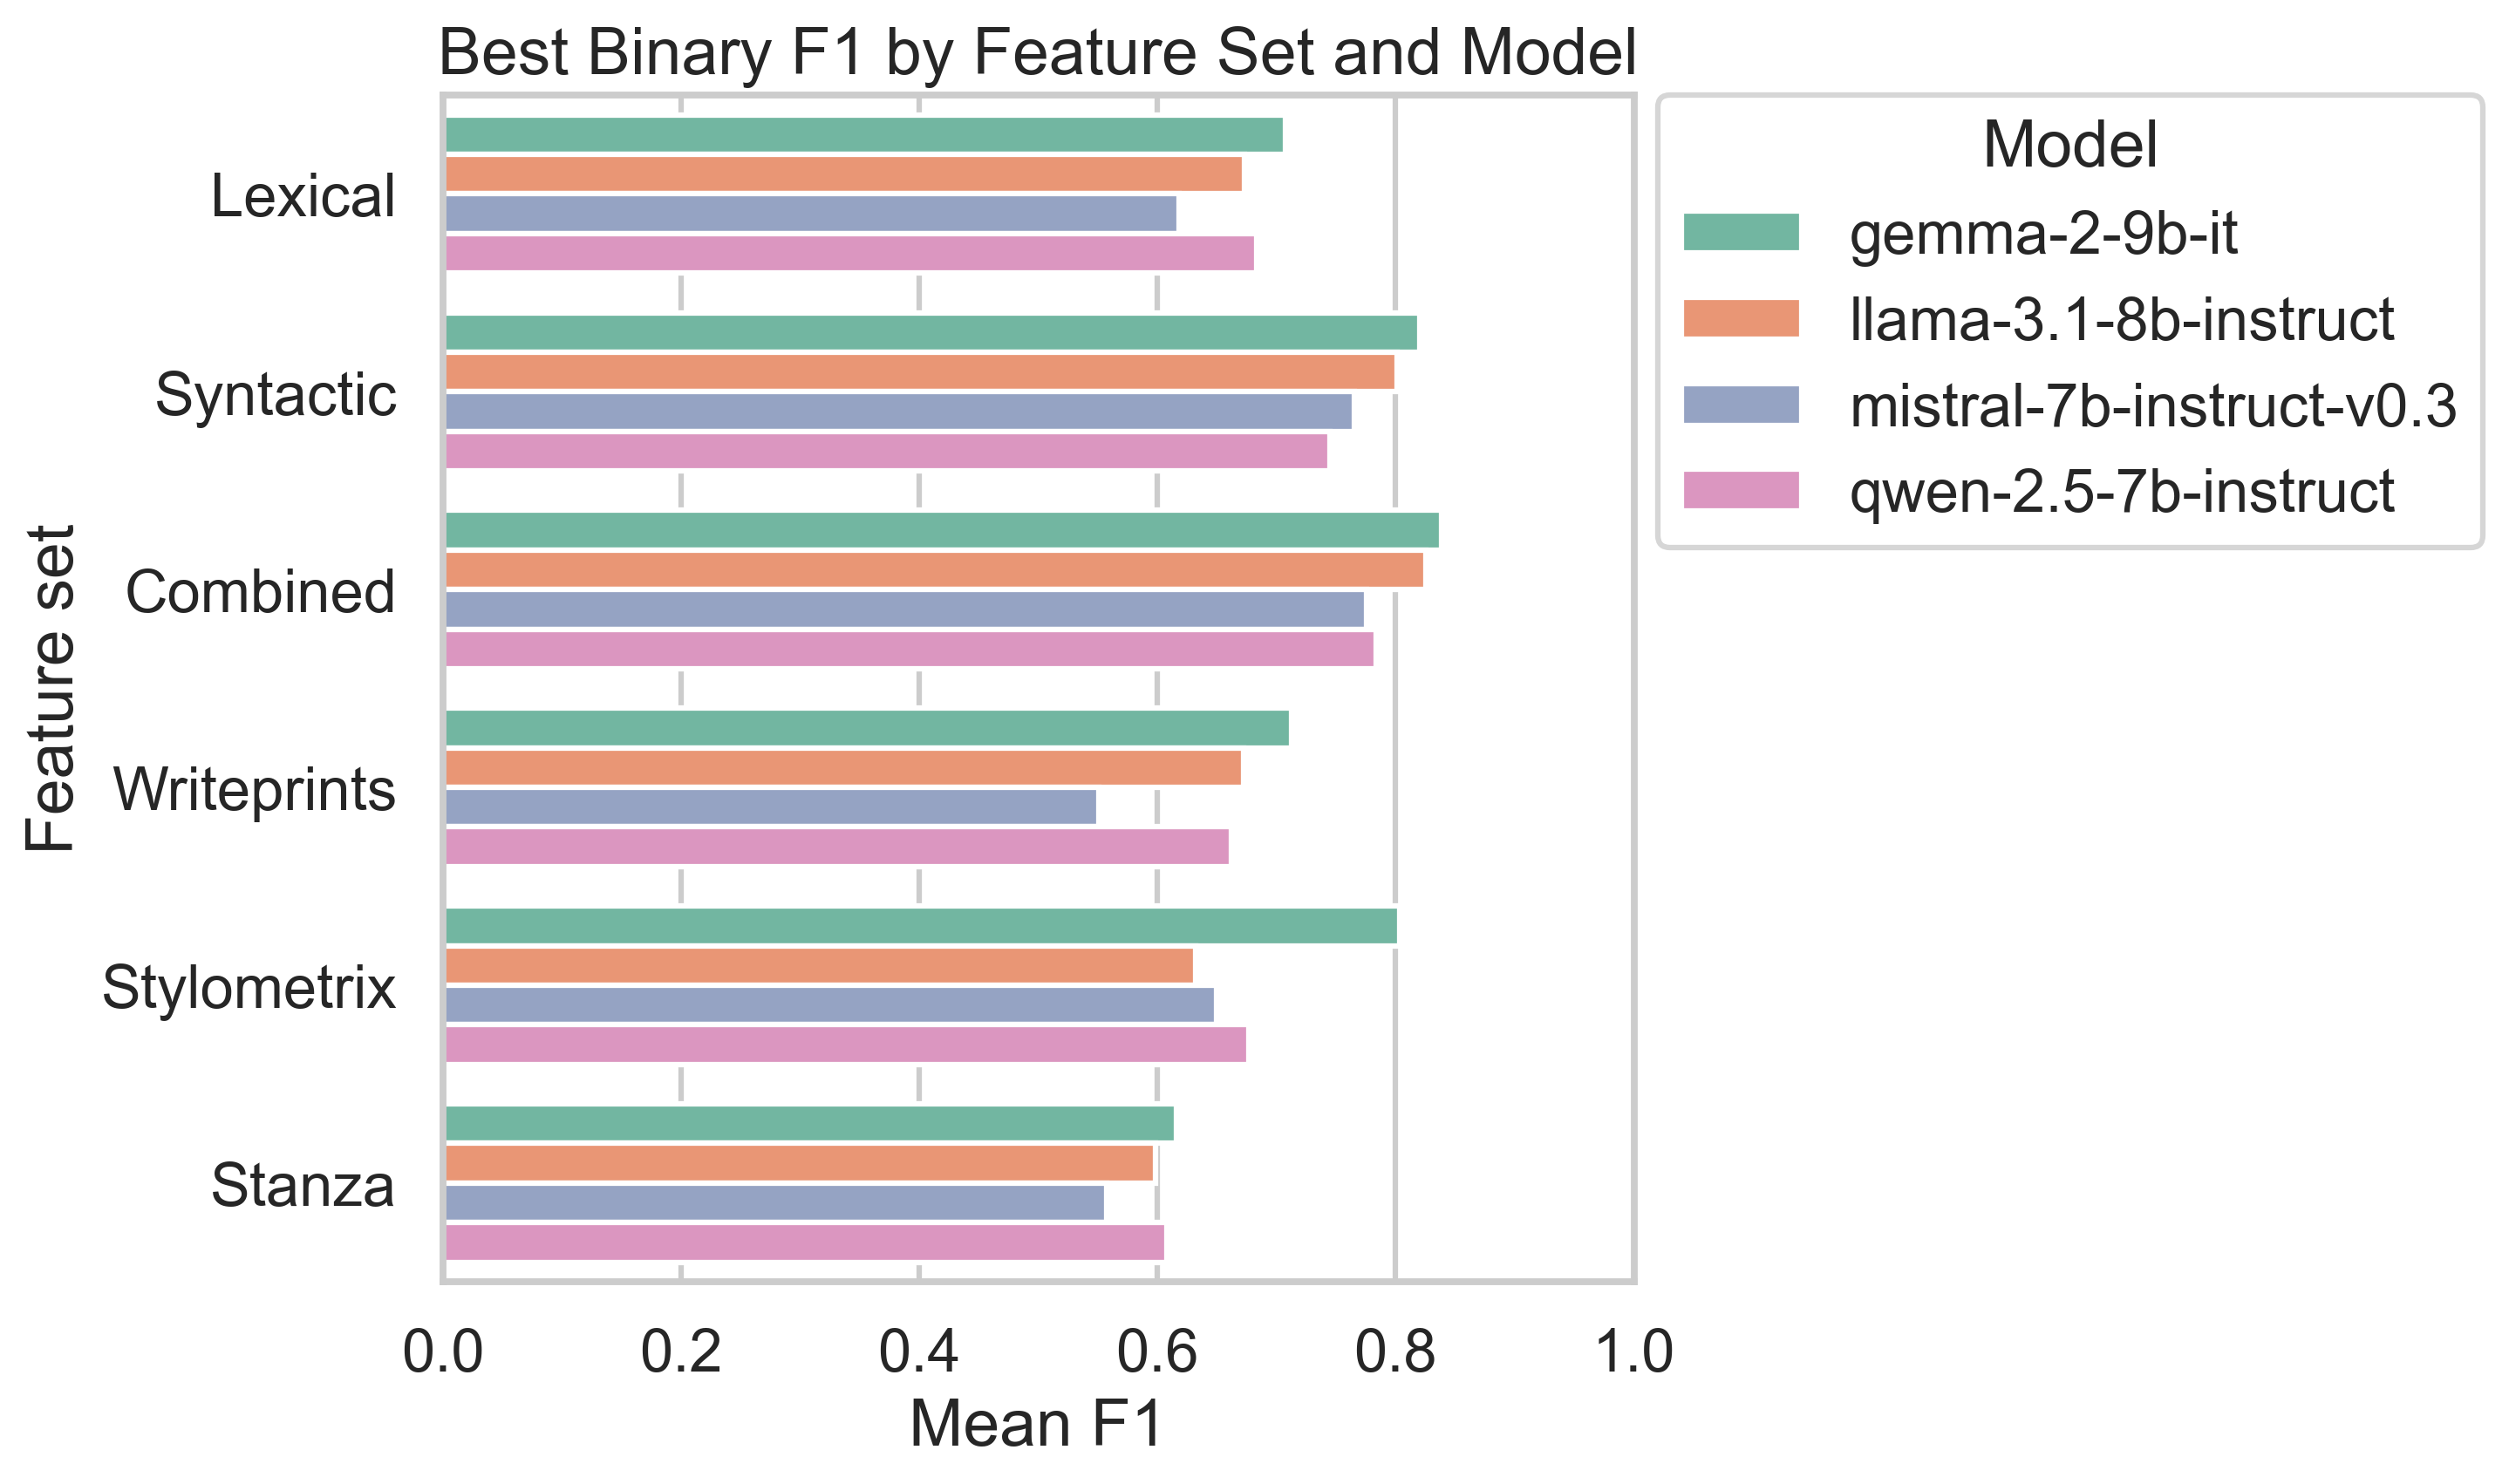
\includegraphics[width=0.9\textwidth]{results/v2/figures/binary_best_f1_by_model.png}
\caption{Best binary mean F1-score by feature set and model. Combined and syntactic feature sets dominate the strongest human-versus-model comparisons, especially for Gemma and Llama.}
\label{fig:binary-best-f1}
\end{figure}

\begin{figure}[H]
\centering
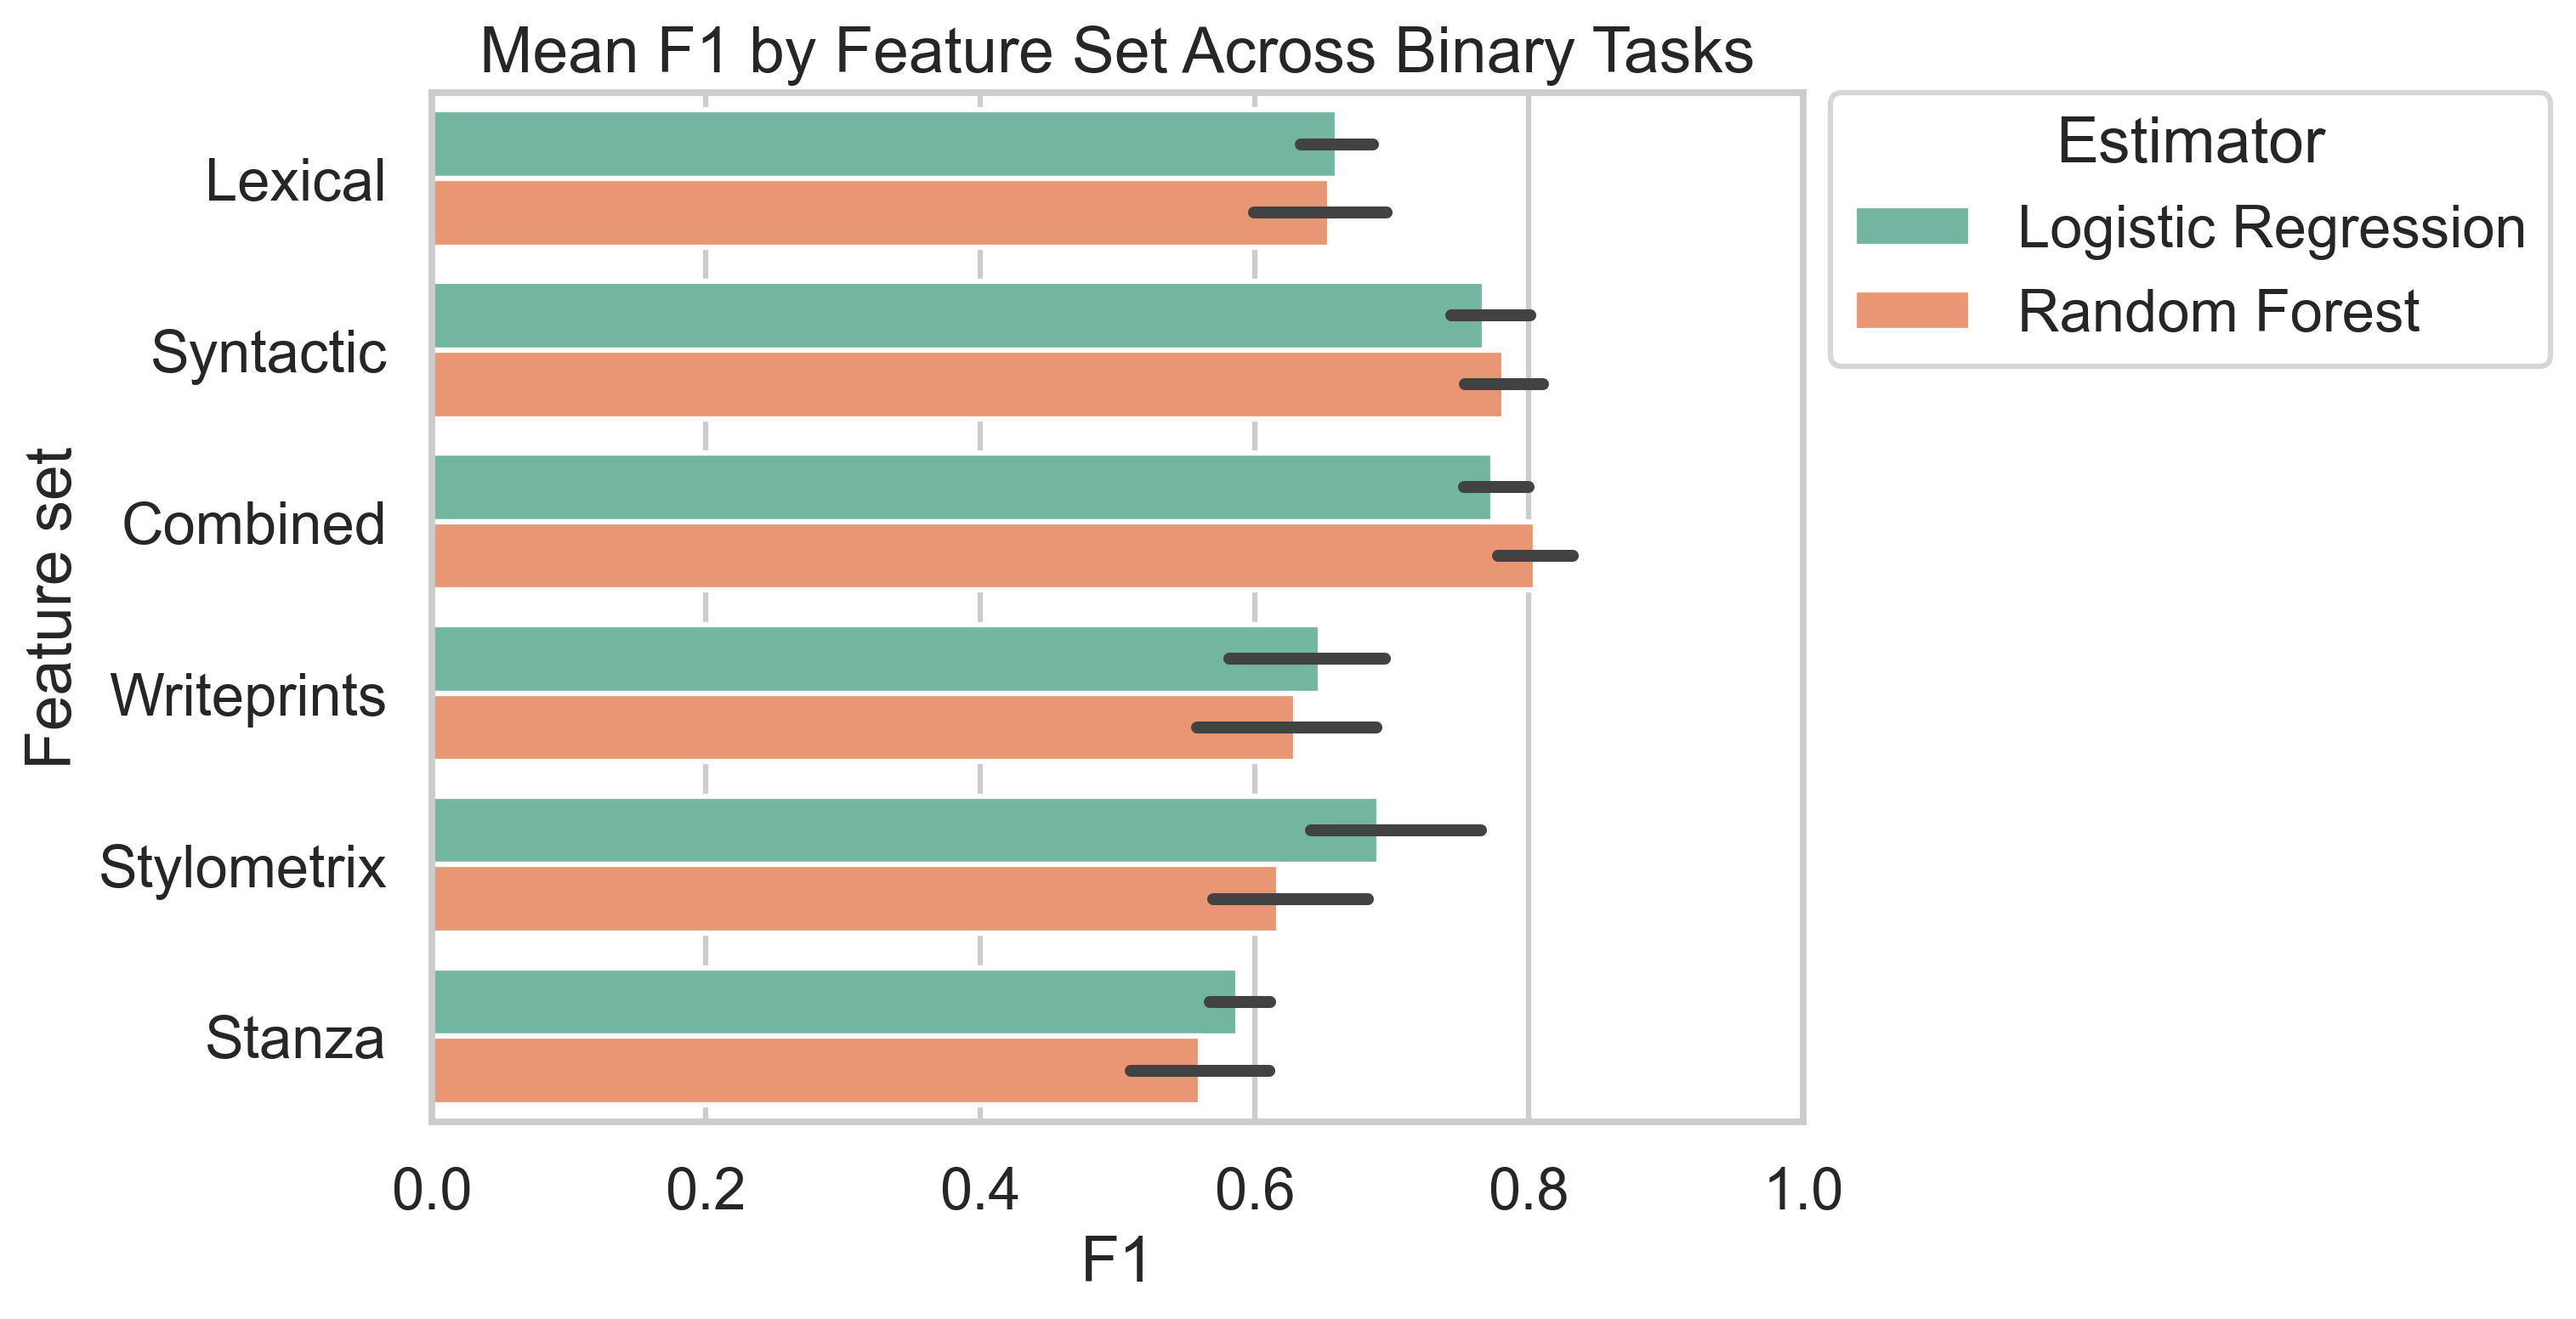
\includegraphics[width=0.9\textwidth]{results/v2/figures/f1_by_feature_set.png}
\caption{Mean binary F1-score by feature set and estimator across the saved binary tasks. Horizontal layout keeps all feature-family labels readable.}
\label{fig:binary-f1-by-feature}
\end{figure}

\subsection{What the Feature Comparison Suggests}

To interpret Figure~\ref{fig:binary-f1-by-feature} clearly, each label corresponds to a different feature set. \texttt{Lexical} refers to vocabulary-based summary measures. \texttt{Syntactic} refers to sentence-structure and related stylistic distribution measures. \texttt{Combined} merges both of those sets. \texttt{Writeprints}, \texttt{stylometrix}, and \texttt{stanza} are lightweight proxy feature families designed to capture additional stylistic patterns, but they are not full implementations of those named toolkits. Figure~\ref{fig:binary-f1-by-feature} therefore compares six distinct ways of representing writing style, from simple lexical summaries through to broader structural and proxy-based feature spaces.

Lexical-only features are consistently weaker than the best combined and syntactic settings. This is methodologically plausible. Because the LLM rewrites are based on the same source abstracts, strong lexical overlap is expected. Human and generated texts operate in the same academic domain and discuss the same underlying research topics. That limits the discriminative value of simple vocabulary-based measures.

Syntactic and combined features perform better because they capture how ideas are arranged rather than which content words are selected. Function-word distributions, sentence-length behaviour, punctuation patterns, and related structural cues are less directly tied to source-topic overlap. This helps explain why combined and syntactic feature sets dominate the stronger binary results across multiple models.

The proxy feature families produce mixed outcomes. \texttt{Stylometrix} performs strongly for the Gemma binary task, where Logistic Regression with this feature family reaches mean F1 of 0.7965, making it competitive with some higher-performing lexical and writeprints configurations. \texttt{Writeprints} tends to occupy a middle range: clearly behind the strongest combined and syntactic settings, but often stronger than \texttt{stanza}. \texttt{Stanza} is consistently the weakest family in the current result set, both in binary and multiclass settings.

\begin{figure}[H]
\centering
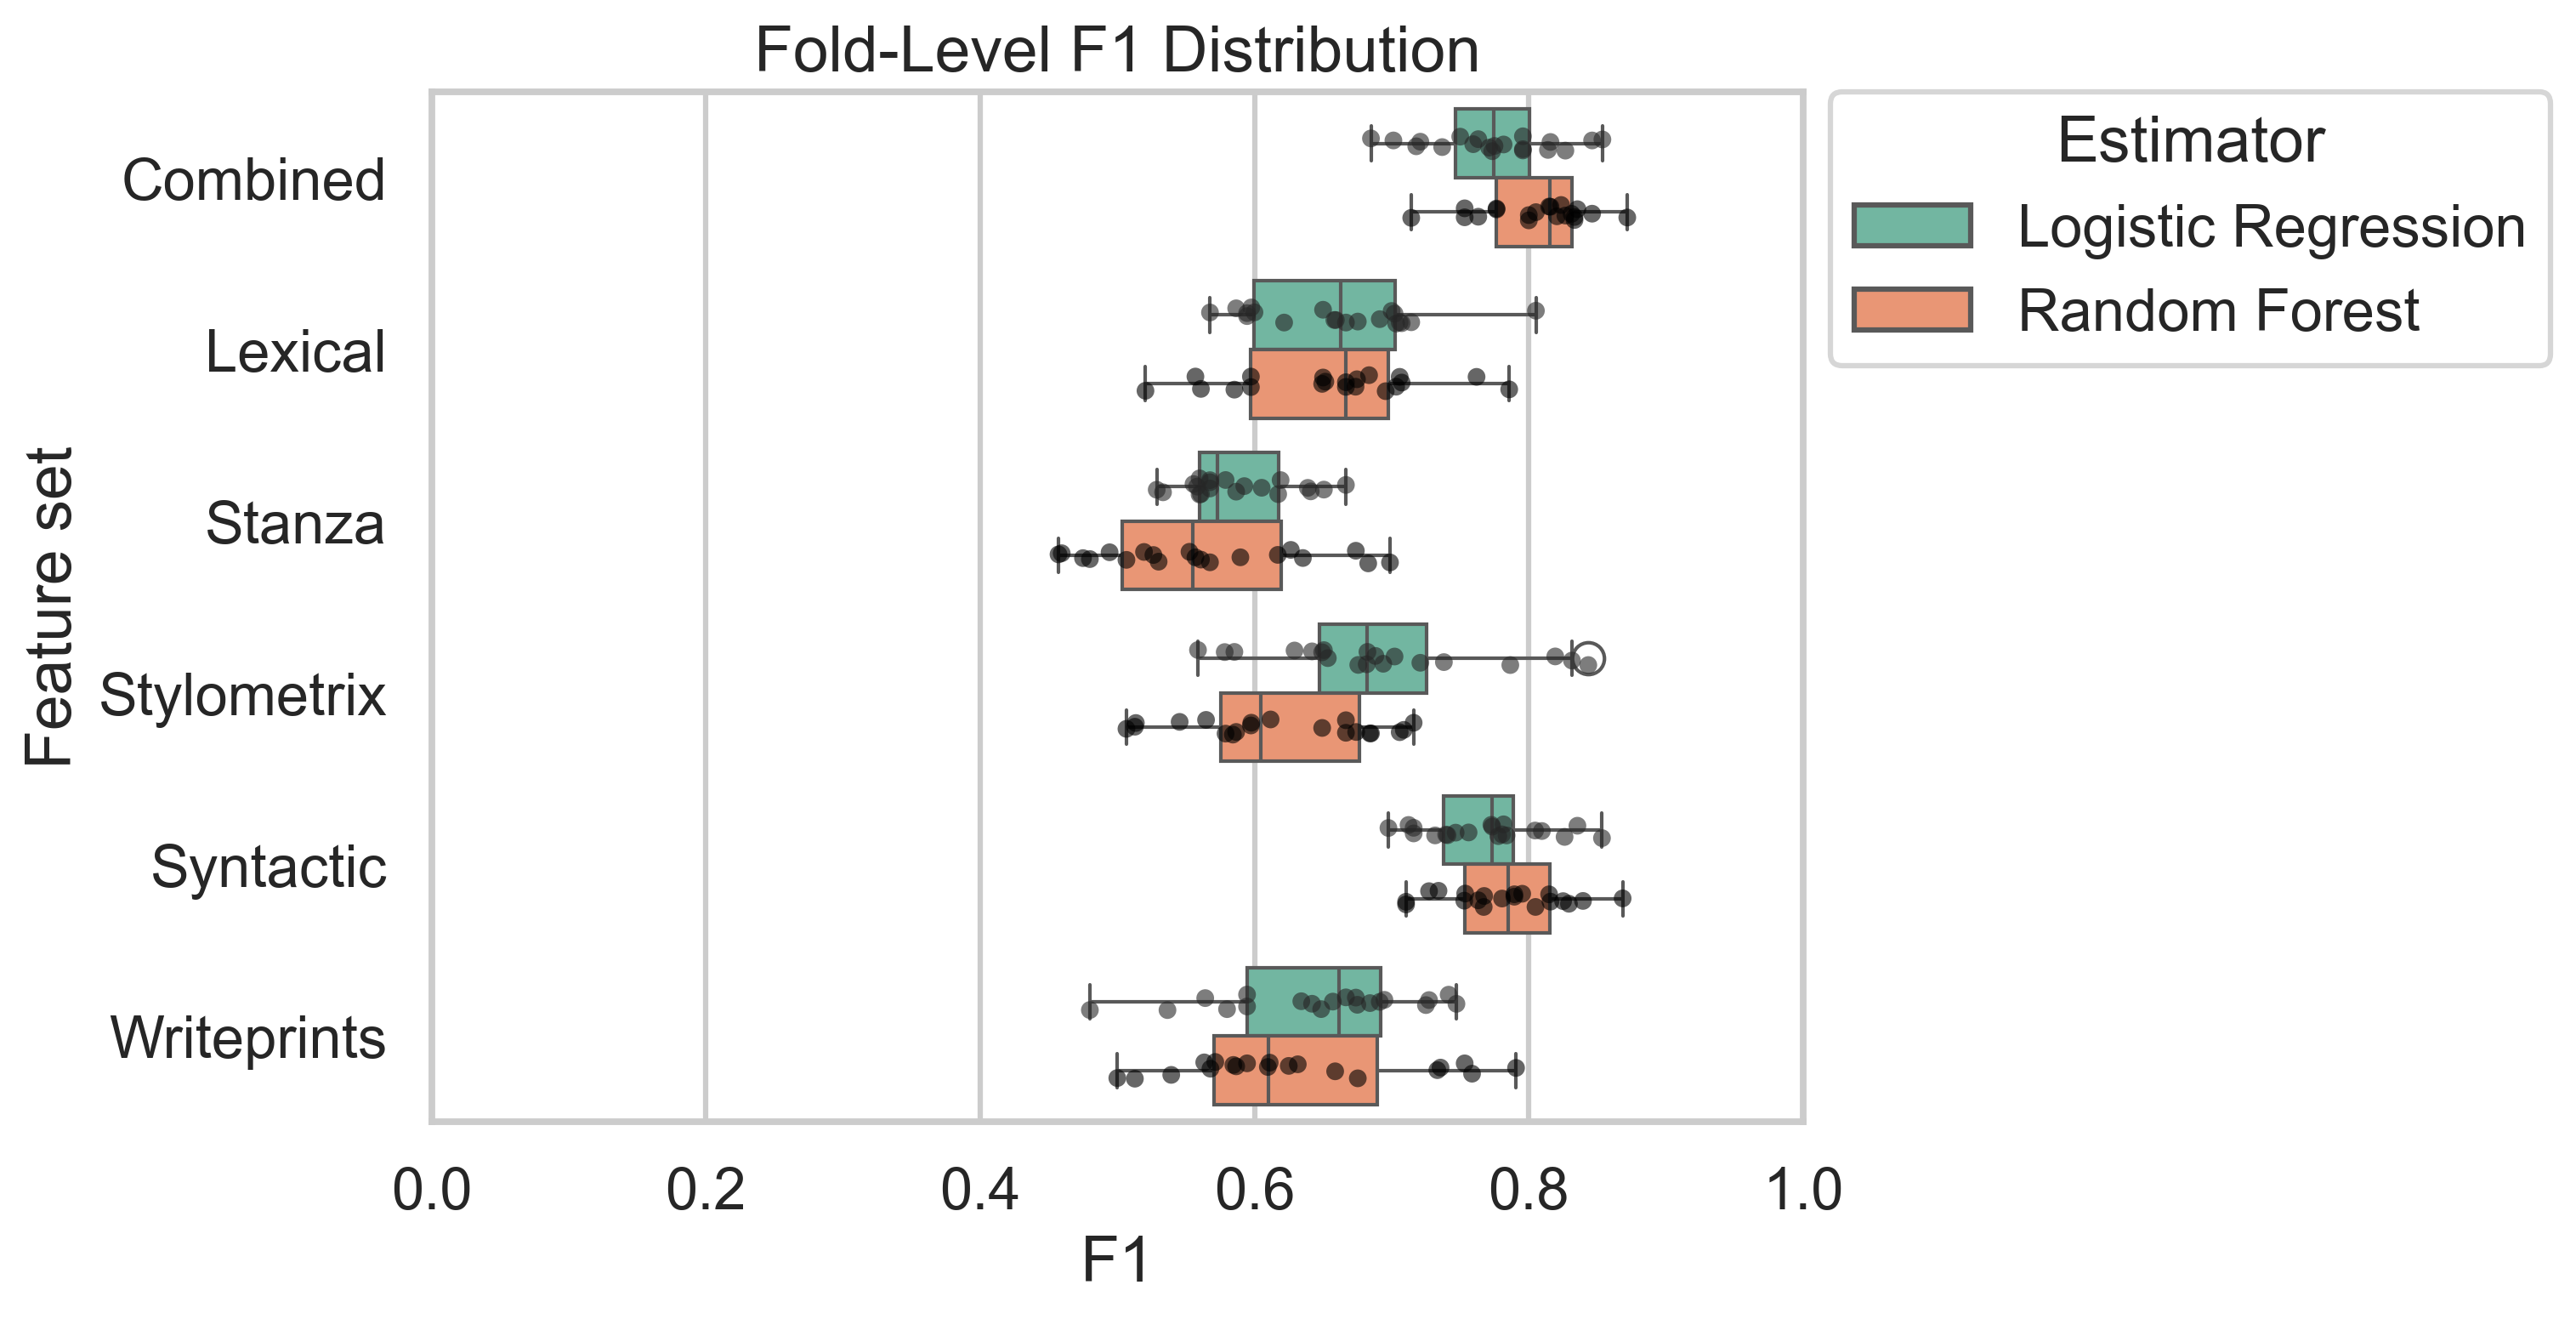
\includegraphics[width=0.9\textwidth]{results/v2/figures/f1_fold_distribution.png}
\caption{Fold-level F1-score distribution across binary feature sets and estimators. Lexical and stanza configurations are generally weaker and less reliable than the strongest combined and syntactic settings.}
\label{fig:f1-fold-distribution}
\end{figure}

\subsection{Multiclass Attribution Performance}

The multiclass results are more difficult than the binary tasks, as expected. A single classifier must distinguish among five labels: \texttt{human}, \texttt{llama-3.1-8b-instruct}, \texttt{gemma-2-9b-it}, \texttt{qwen-2.5-7b-instruct}, and \texttt{mistral-7b-instruct-v0.3}. The best multiclass result is Random Forest with combined features, with mean accuracy of 0.506, mean macro-F1 of 0.5053, mean ROC-AUC of 0.8154, and mean MCC of 0.3848. The next best configurations are combined Logistic Regression and syntactic Random Forest.

Although these values are lower than the strongest binary results, they are still informative. Random guessing over five balanced classes would produce much worse performance. The results therefore indicate that the pipeline is learning meaningful class structure, but that distinguishing among multiple LLM families is considerably harder than separating one model from the human class.

The multiclass ordering broadly mirrors the binary findings. Combined and syntactic feature sets remain strongest. Lexical and writeprints-based multiclass models occupy a weaker middle range, stylometrix remains modest, and stanza is weakest. This consistency strengthens the interpretation that structural style signals are the most reliable evidence source in the current pipeline.

\begin{figure}[H]
\centering
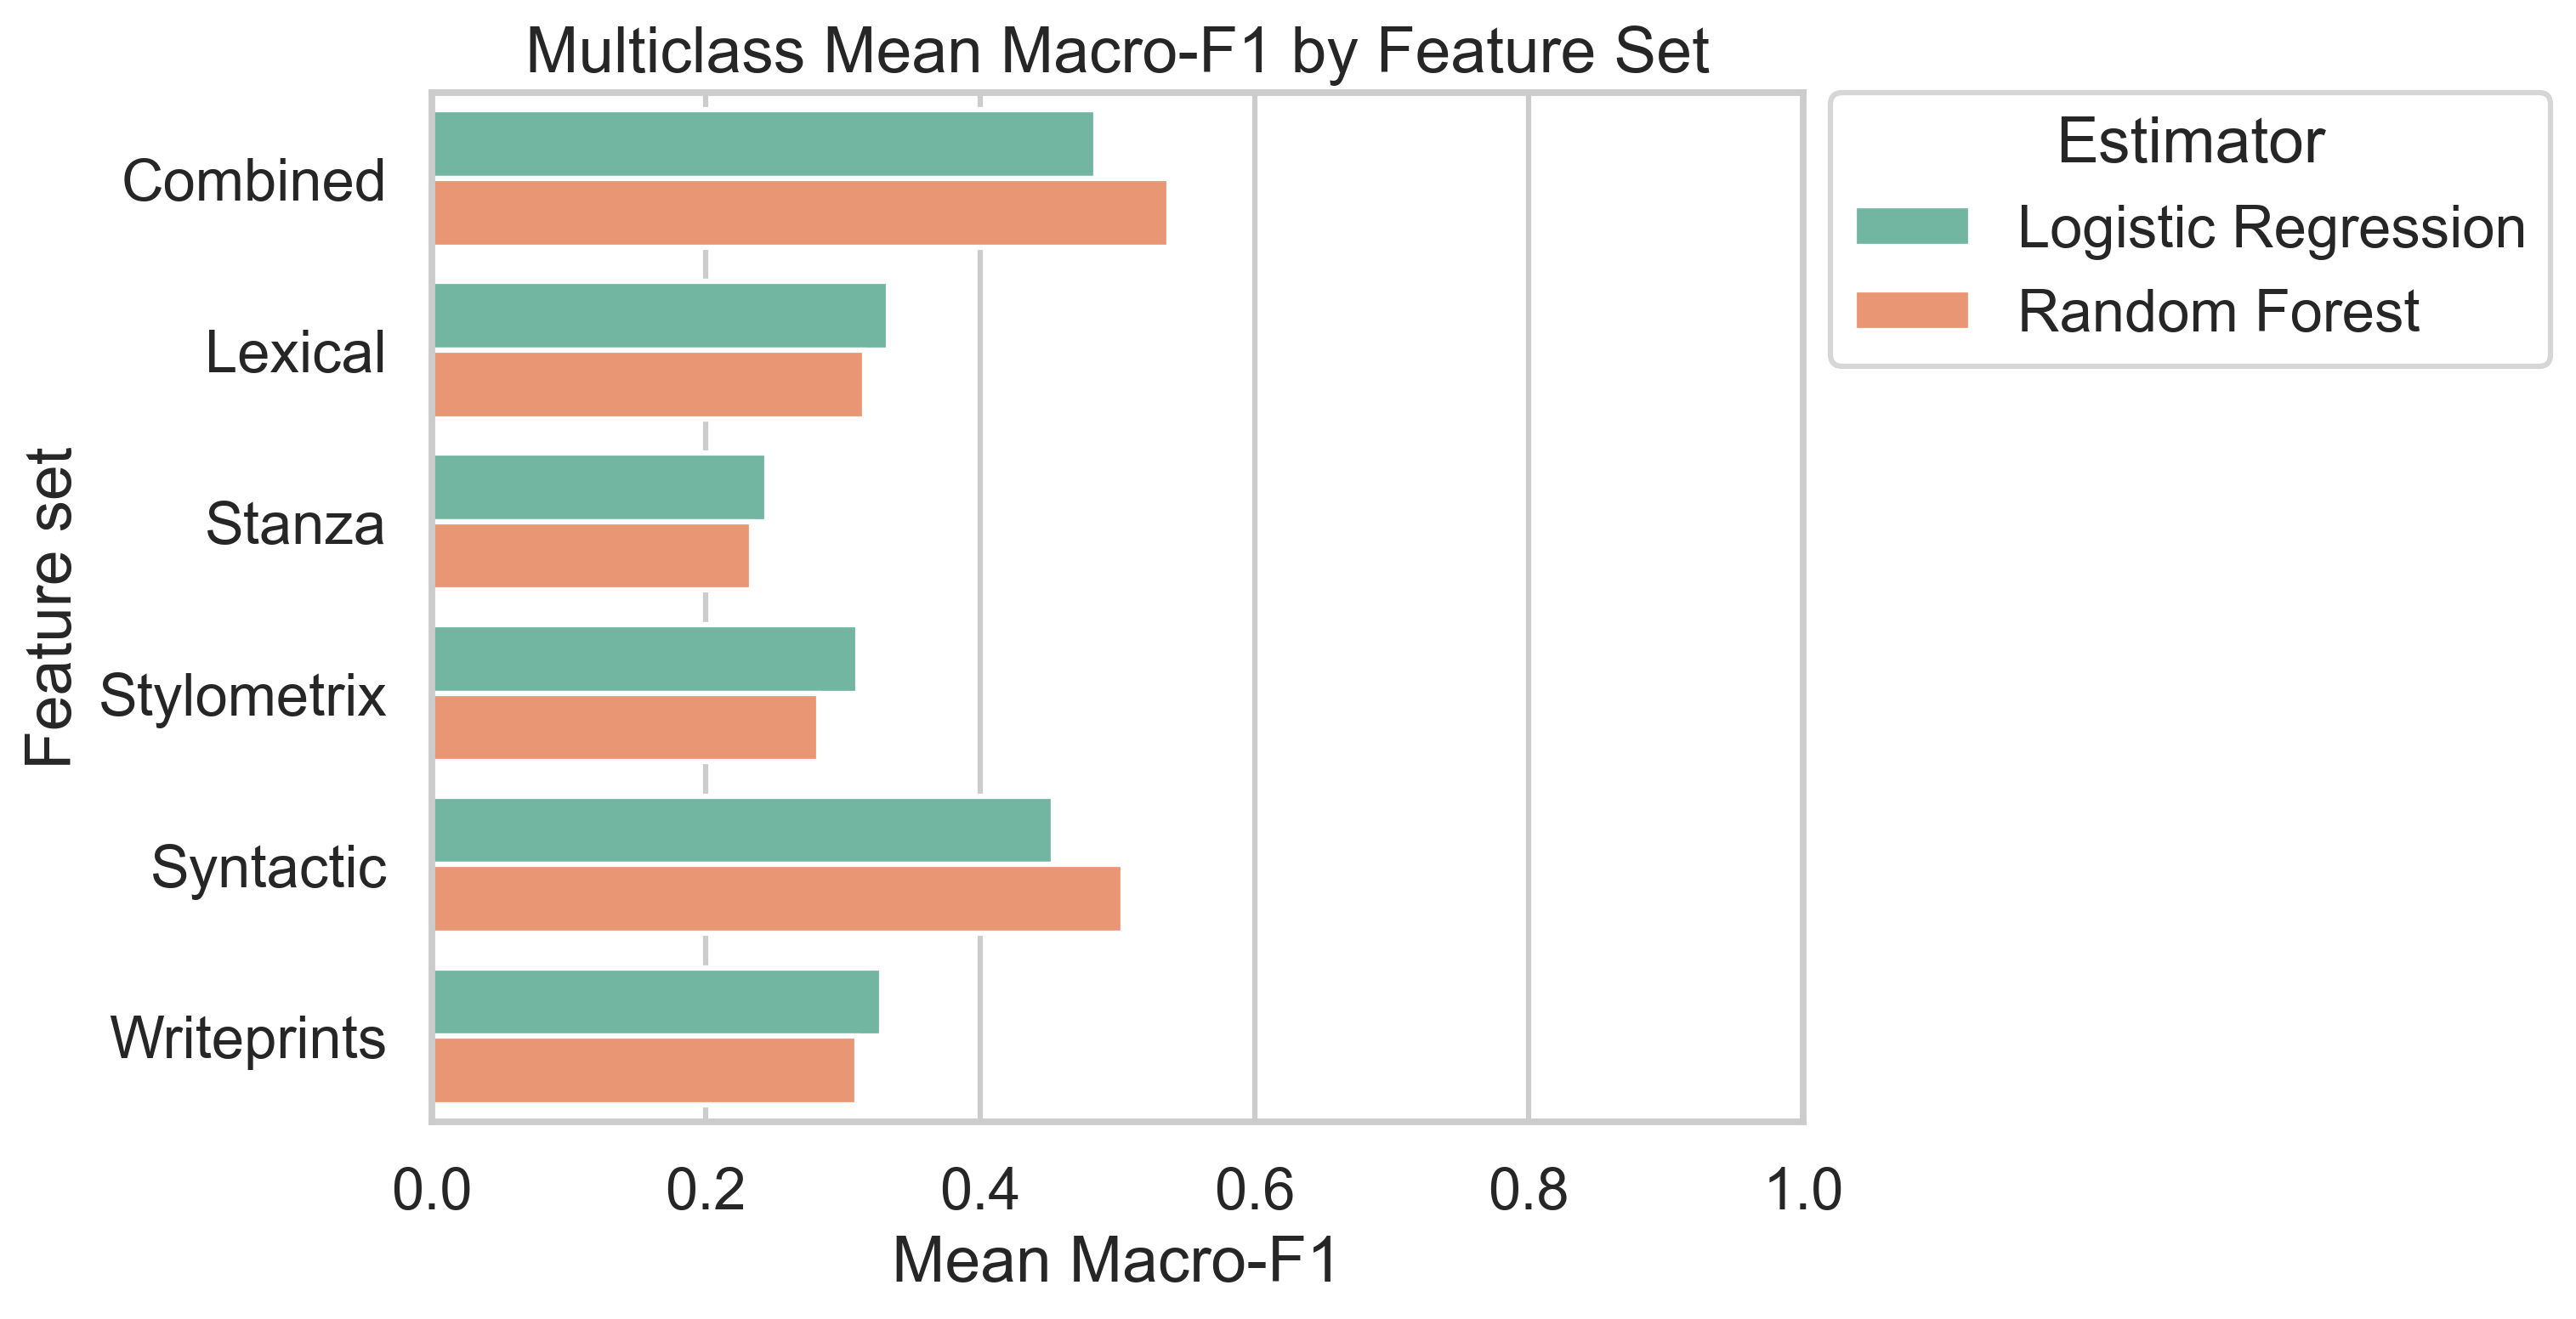
\includegraphics[width=0.9\textwidth]{results/v2/figures/multiclass_f1_mean.png}
\caption{Multiclass mean macro-F1 by feature set and estimator. Combined and syntactic configurations are clearly stronger than lexical, writeprints, stylometrix, and stanza-based alternatives.}
\label{fig:multiclass-f1}
\end{figure}

\subsection{Semantic Overlap Between Human and Generated Abstracts}

The semantic-overlap outputs complement the stylometric analysis by checking whether generated abstracts remain close to their source texts at the content-overlap level. This matters because the stylometric findings are more persuasive if the human and generated texts are semantically aligned rather than topically divergent. Table~\ref{tab:semantic-summary} summarises the saved model-level semantic results.

\begin{table}[H]
\centering
\small
\begin{tabularx}{\textwidth}{>{\raggedright\arraybackslash}p{4.6cm} *{4}{>{\centering\arraybackslash}p{2cm}}}
\toprule
Model & ROUGE-1 F1 & ROUGE-2 F1 & ROUGE-L F1 & METEOR \\
\midrule
\texttt{llama-3.1-8b-instruct} & 0.6958 & 0.4589 & 0.5688 & 0.6306 \\
\texttt{gemma-2-9b-it} & 0.6281 & 0.3529 & 0.4914 & 0.5356 \\
\texttt{qwen-2.5-7b-instruct} & 0.6305 & 0.3688 & 0.5222 & 0.5482 \\
\texttt{mistral-7b-instruct-v0.3} & 0.7346 & 0.5174 & 0.6527 & 0.6879 \\
\bottomrule
\end{tabularx}
\caption{Mean semantic-overlap scores by model. METEOR is a simplified in-project implementation rather than the official toolkit version.}
\label{tab:semantic-summary}
\end{table}

These scores indicate that all four LLMs preserve substantial content overlap with the human source abstracts. Mistral produces the highest average overlap on all four saved semantic measures, while Llama is the next strongest. Gemma and Qwen are lower, but still well above trivial overlap levels. This matters for interpretation: the binary and multiclass stylometric results cannot be dismissed as purely topic-driven because the generated texts are still recognisably close to the original abstract content. In other words, the project now shows both semantic alignment and stylistic separability.

The semantic results should still be interpreted cautiously. ROUGE and METEOR-style scores are overlap-oriented and do not prove deep semantic equivalence. They are most useful here as a supporting validity check. Their value lies in showing that the human and generated texts are not unrelated rewrites or off-topic generations, which strengthens the argument that the classifiers are responding to stylistic differences rather than obvious content drift.

\subsection{Analysis Result Summary}

The updated result set supports a stronger answer to the first two research questions than the earlier partial-result version of the report did. The pipeline now demonstrates human-versus-model separation across all four configured LLMs, provides multiclass evidence across the full five-class setting, and includes semantic-overlap outputs showing that generated texts remain substantially aligned with the source abstracts. The strongest results consistently come from combined and syntactic feature spaces, which is a coherent and repeatable pattern rather than a one-off outcome.

However, the current evidence still does not justify stronger claims such as universal LLM stylometric detectability, domain-independent generalisation, or forensic-level certainty. The study remains limited to one domain, one language, and one prompt condition. The proxy feature families also still need stronger validation. These are meaningful pilot results, but they are not yet a complete benchmark.

\section{Discussion and Conclusions}

\subsection{Answers to the Research Questions}

The first research question asked whether feature-based stylometry can distinguish human-written academic abstracts from LLM-generated rewrites of the same source papers. Based on the updated outputs, the answer is yes. All four binary human-versus-model tasks show learnable separation, with the strongest results observed for Gemma and Llama.

The second research question asked which feature families are most informative. The updated evidence clearly indicates that combined and syntactic feature sets are the strongest overall. Lexical features are weaker, stanza is the weakest family, and writeprints and stylometrix occupy a middle position with model-dependent usefulness.

The third research question asked what can be concluded from the current outputs about multiclass attribution. The most defensible conclusion is that the pipeline supports meaningful multiclass separation across the five balanced classes, but that this is substantially harder than the binary tasks. Combined Random Forest is the strongest multiclass configuration, with mean macro-F1 just above 0.50.

The supporting semantic question can also now be answered. The ROUGE and simplified METEOR outputs show that the generated texts remain meaningfully aligned with their source abstracts, especially for Mistral and Llama. This makes the stylometric findings stronger, because the classifiers are separating texts that remain semantically close rather than trivially different in topic or information content.

These answers should still be interpreted in relation to the limitations of the project. The study is based on one academic domain, one language, one prompt condition, and a relatively small balanced pilot subset. In addition, some of the feature families are proxy implementations rather than full external toolkits, and the semantic evaluation is overlap-based rather than a deep measure of meaning. For these reasons, the discussion supports a careful claim about stylistic separability in this specific controlled setting, but it does not justify stronger claims about universal LLM detection or forensic-level certainty across all writing contexts.

\subsection{Conclusions (Take-away Messages)}

This project shows that feature-based stylometry can separate human-written academic abstracts from LLM-generated rewrites in a controlled, source-matched setting. The strongest results come from combined and syntactic feature sets, not from lexical richness alone. This indicates that the main stylistic signal is structural rather than purely vocabulary-based.

The updated local result set strengthens the report substantially. It now includes all four binary model comparisons, multiclass outputs for all six configured feature families, and model-level semantic-overlap summaries. The strongest binary result is Gemma with syntactic features and Logistic Regression (mean F1 = 0.8276), while the strongest multiclass result is combined Random Forest (mean macro-F1 = 0.5053). The semantic results show that generated texts remain close to their sources, with Mistral achieving the highest overlap values across ROUGE-1, ROUGE-L, and simplified METEOR.

The main limitation is that the study remains a pilot. It is domain-specific, prompt-specific, and partly dependent on proxy feature families that still need stronger validation. The semantic evaluation is also lightweight: ROUGE is overlap-based, and the METEOR score implemented here is a simplified in-project variant rather than a direct toolkit reproduction. The results are credible and informative, but they should not be overstated as universal evidence about all LLM writing detection scenarios.

This also implies that different prompt engineering methods, such as few-shot prompting or other prompt types, might influence the credibility of the generated abstracts and cause different stylometric patterns within the same model. Future work should therefore test newer and more capable model families rather than assuming that the patterns observed here will transfer unchanged. Even so, the current evidence supports the view that LLM outputs can retain textual properties that lead to distinguishable judgements by stylometric analysis (Zaitsu et al., 2025).

The main next steps are clear. First, the proxy feature families should be validated more carefully or replaced with direct toolkit integrations. Second, the experiment should be extended beyond factual prompt rewrites into additional prompt conditions and domains. Third, the analysis should be strengthened with more explicit interpretability outputs, such as per-feature importance summaries and structured error analysis across models.

\subsection{Personal Lessons Learned (What I Personally Gained from the Project)}

This project taught me that useful stylometric analysis depends on more than choosing a classifier. Corpus design, leakage control, feature selection, and careful interpretation are just as important, and using grouped cross-validation by \texttt{source\_id} showed how easily results can be overstated when the evaluation design is weak. I also learned that strong research requires justified methodological decisions, honest limitations, and evidence that is not stretched beyond what it supports. The config-driven workflow reinforced the value of reproducibility because it made the analysis easier to rerun, inspect, and improve. Finally, practical issues such as HPC constraints, storage limits, dependencies, and execution failures showed me that applied research requires patience, adaptability, and systematic problem-solving as well as technical knowledge.

\section{References}

\begin{hangparas}{2em}{1}

Banerjee, S., \& Lavie, A. (2005). METEOR: An automatic metric for MT evaluation with improved correlation with human judgments. \textit{Proceedings of the ACL Workshop on Intrinsic and Extrinsic Evaluation Measures for Machine Translation and/or Summarization}, 65--72. \url{https://aclanthology.org/W05-0909/}

Dhaini, M., Poelman, W., \& Erdogan, E. (2023). Detecting ChatGPT: A Survey of the State of Detecting ChatGPT-Generated Text. \textit{ArXiv (Cornell University)}. \url{https://doi.org/10.48550/arxiv.2309.07689}

Erol, G., Ergen, A., Erol, B. G., Ergen, S. K., Bora, T. S., Colgecen, A. D., Araz, B., Sahin, C., Bostanci, G., Kilic, I., Macit, Z. B., Sevgi, U. T., \& Gungor, A. (2025). Can we trust academic AI detective? Accuracy and limitations of AI-output detectors. \textit{Acta Neurochirurgica, 167}(1). \url{https://doi.org/10.1007/s00701-025-06622-4}

Geng, M., \& Trotta, R. (2024, April 12). Is ChatGPT Transforming Academics' Writing Style? \textit{ArXiv.org}. \url{https://doi.org/10.48550/arXiv.2404.08627}

Holmes, D. I., \& Kardos, J. (2003). Who Was the Author? An Introduction to Stylometry. \textit{CHANCE, 16}(2), 5--8. \url{https://doi.org/10.1080/09332480.2003.10554842}

Huang, J., \& Tan, M. (2023). The role of ChatGPT in scientific communication: Writing better scientific review articles. \textit{American Journal of Cancer Research, 13}(4), 1148. \url{https://pmc.ncbi.nlm.nih.gov/articles/PMC10164801/}

Jockers, M. L., \& Witten, D. M. (2010). A comparative study of machine learning methods for authorship attribution. \textit{Literary and Linguistic Computing, 25}(2), 215--223. \url{https://doi.org/10.1093/llc/fqq001}

Koppel, M., Schler, J., \& Argamon, S. (2009). Computational methods in authorship attribution. \textit{Journal of the American Society for Information Science and Technology, 60}(1), 9--26. \url{https://doi.org/10.1002/asi.20961}

L\'opez-Escobedo, F., M\'endez-Cruz, C.-F., Sierra, G., \& Sol\'orzano-Soto, J. (2013). Analysis of Stylometric Variables in Long and Short Texts. \textit{Procedia - Social and Behavioral Sciences, 95}, 604--611. \url{https://doi.org/10.1016/j.sbspro.2013.10.688}

Lin, C.-Y. (2004). ROUGE: A package for automatic evaluation of summaries. \textit{Proceedings of the Workshop on Text Summarization Branches Out}, 74--81. \url{https://aclanthology.org/W04-1013/}

Mikros, G. (2025). Beyond the surface: stylometric analysis of GPT-4o's capacity for literary style imitation. \textit{Digital Scholarship in the Humanities, 40}(2). \url{https://doi.org/10.1093/llc/fqaf035}

Mitchell, E., Lee, Y., Khazatsky, A., Manning, C. D., \& Finn, C. (2023). DetectGPT: Zero-shot machine-generated text detection using probability curvature. \textit{Proceedings of the 40th International Conference on Machine Learning, PMLR 202}, 24950--24962. \url{https://proceedings.mlr.press/v202/mitchell23a.html}

Neal, T., Sundararajan, K., Fatima, A., Yan, Y., Xiang, Y., \& Woodard, D. (2018). Surveying Stylometry Techniques and Applications. \textit{ACM Computing Surveys, 50}(6), 1--36. \url{https://doi.org/10.1145/3132039}

Przystalski, K., Argasi\'nski, J. K., Grabska-Gradzi\'nska, I., \& Ochab, J. K. (2025). Stylometry recognizes human and LLM-generated texts in short samples. \textit{Expert Systems with Applications, 296}, 129001. \url{https://doi.org/10.1016/j.eswa.2025.129001}

Solaiman, I., Brundage, M., Clark, J., Askell, A., Herbert-Voss, A., Wu, J., Radford, A., \& Wang, J. (2019). Release strategies and the social impacts of language models. \textit{ArXiv}. \url{https://doi.org/10.48550/arXiv.1908.09203}


Zaitsu, W., Jin, M., Ishihara, S., Satoru Tsuge, \& Inaba, M. (2025). Stylometry can reveal artificial intelligence authorship, but humans struggle: A comparison of human and seven large language models in Japanese. \textit{PLoS ONE, 20}(10), e0335369--e0335369. \url{https://doi.org/10.1371/journal.pone.0335369}

Zheng, R., Li, J., Chen, H., \& Huang, Z. (2006). A framework for authorship identification of online messages: Writing-style features and classification techniques. \textit{Journal of the American Society for Information Science and Technology, 57}(3), 378--393. \url{https://doi.org/10.1002/asi.20316}

\end{hangparas}

\section{Appendix}

\subsection{Ethical Approval Form}

\begin{figure}[H]
\centering
\fbox{
\includegraphics[width=0.9\textwidth]{ethical_form_ss.png}}
\end{figure}

\subsection{Additional Supporting Information}

This appendix contains supporting material that was useful for checking the research pipeline but was not included in the main report. The figures and tables below are supplementary rather than repeated versions of the main evidence.

\subsubsection{Configuration Evidence}

\begin{figure}[H]
\centering
\fbox{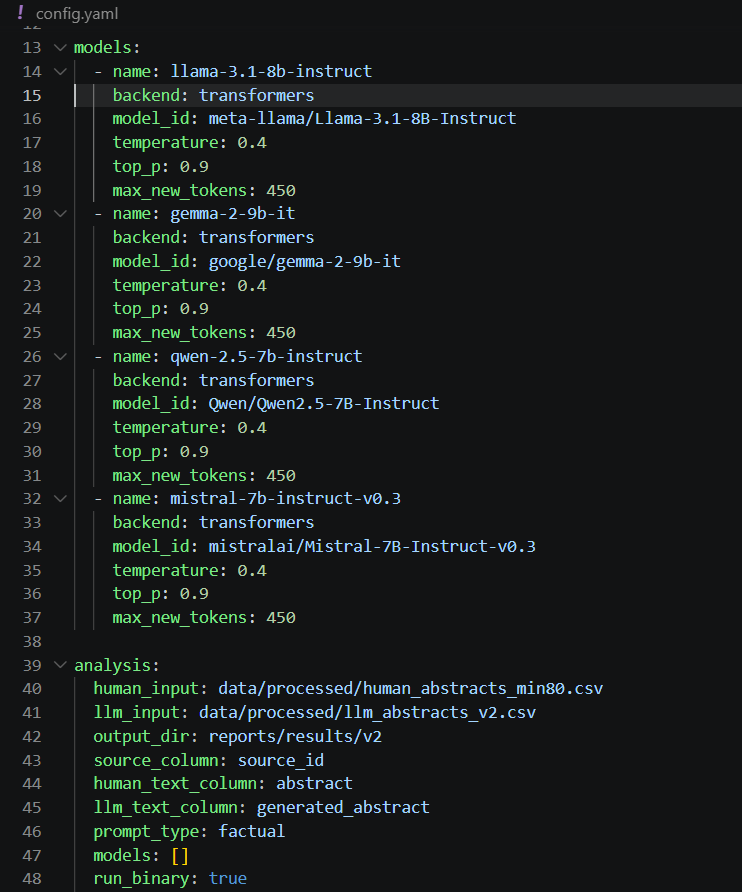
\includegraphics[width=0.92\textwidth]{config.png}}
\caption{Configuration screenshot showing the four LLM families and the analysis settings used in the reproducible pipeline.}
\label{fig:appendix-config}
\end{figure}

\begin{table}[H]
\centering
\scriptsize
\begin{tabularx}{\textwidth}{lXccc}
\toprule
Model label & Model identifier & Temperature & Top-p & Max tokens \\
\midrule
Llama & \texttt{meta-llama/Llama-3.1-8B-Instruct} & 0.4 & 0.9 & 450 \\
Gemma & \texttt{google/gemma-2-9b-it} & 0.4 & 0.9 & 450 \\
Qwen & \texttt{Qwen/Qwen2.5-7B-Instruct} & 0.4 & 0.9 & 450 \\
Mistral & \texttt{mistralai/Mistral-7B-Instruct-v0.3} & 0.4 & 0.9 & 450 \\
\bottomrule
\end{tabularx}
\caption{Generation configuration for the four LLM families. The shared decoding settings help keep the comparison focused on model and style differences rather than deliberately different sampling parameters.}
\label{tab:appendix-model-config}
\end{table}

\begin{table}[H]
\centering
\small
\begin{tabularx}{\textwidth}{lX}
\toprule
Setting & Value \\
\midrule
Human input & \texttt{data/processed/human\_abstracts\_min80.csv} \\
LLM input & \texttt{data/processed/llm\_abstracts\_v2.csv} \\
Analysis output & \texttt{reports/results/v2} \\
Source grouping key & \texttt{source\_id} \\
Human text column & \texttt{abstract} \\
LLM text column & \texttt{generated\_abstract} \\
Prompt type & \texttt{factual} \\
Cross-validation & 5-fold grouped cross-validation \\
Random seed & 42 \\
Feature families & lexical, syntactic, combined, writeprints, stylometrix, stanza \\
\bottomrule
\end{tabularx}
\caption{Analysis configuration used to generate the main result files.}
\label{tab:appendix-analysis-config}
\end{table}

\subsubsection{Supplementary Result Figures}

\begin{figure}[H]
\centering
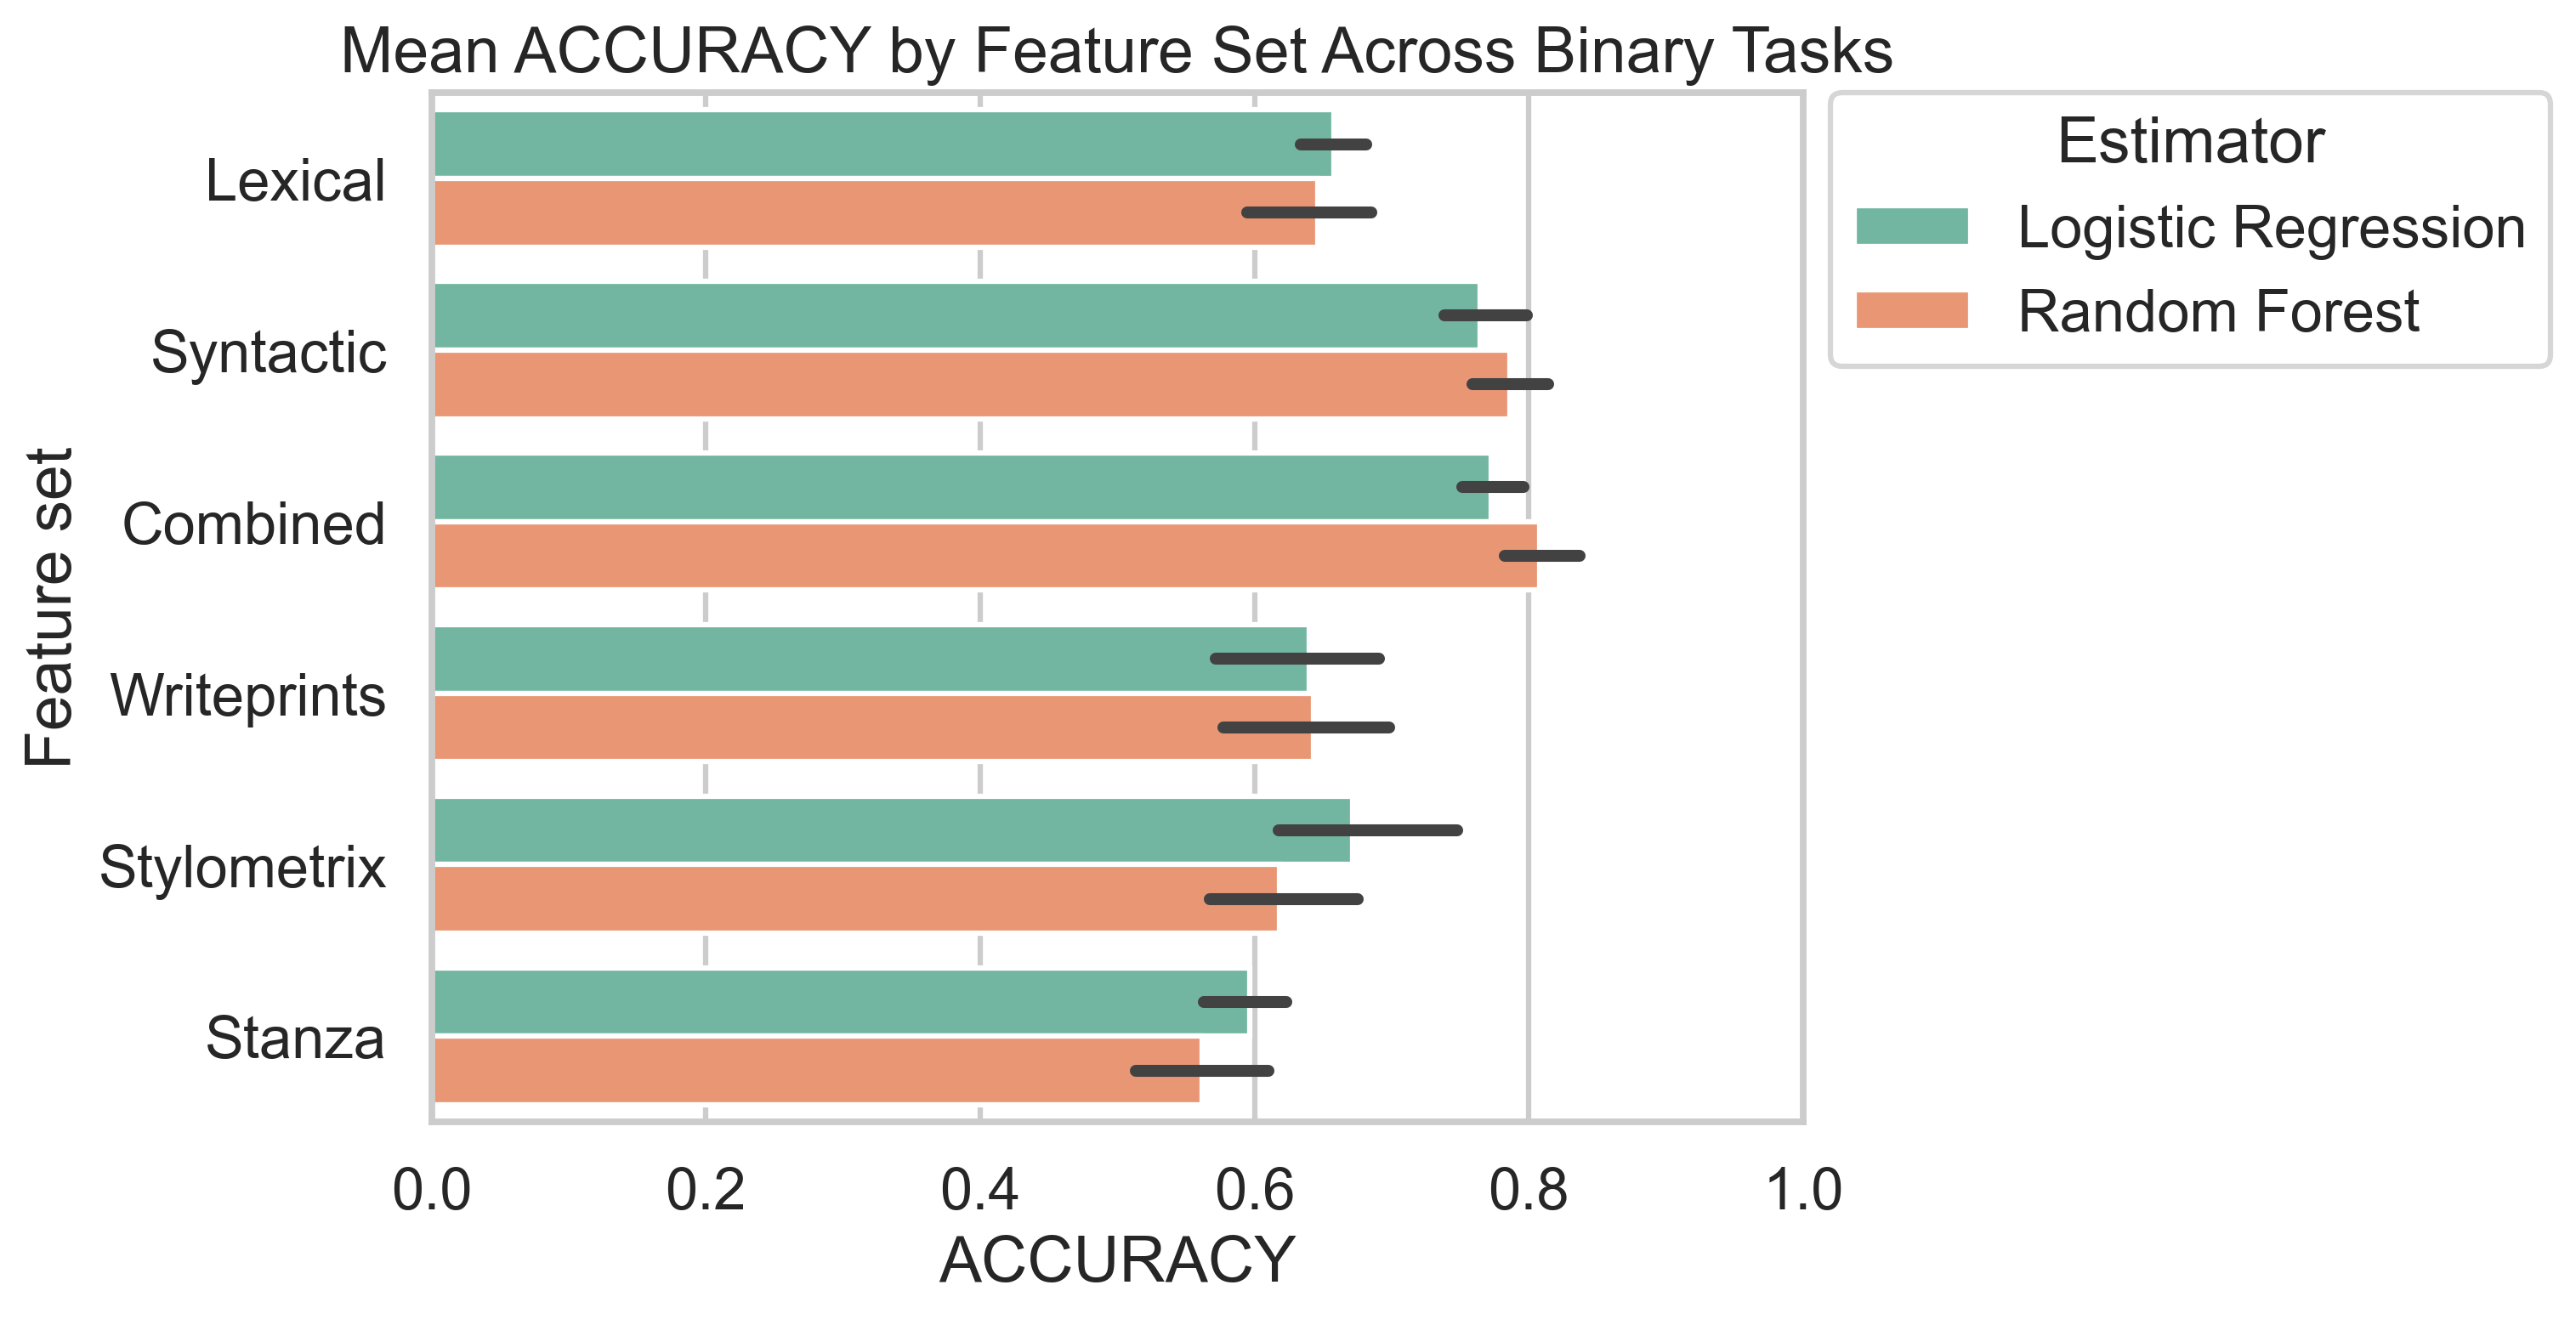
\includegraphics[width=0.9\textwidth]{results/v2/figures/accuracy_by_feature_set.png}
\caption{Supplementary binary mean accuracy by feature set and estimator. This complements the F1-focused figures in the main report.}
\label{fig:appendix-accuracy-feature}
\end{figure}

\begin{figure}[H]
\centering
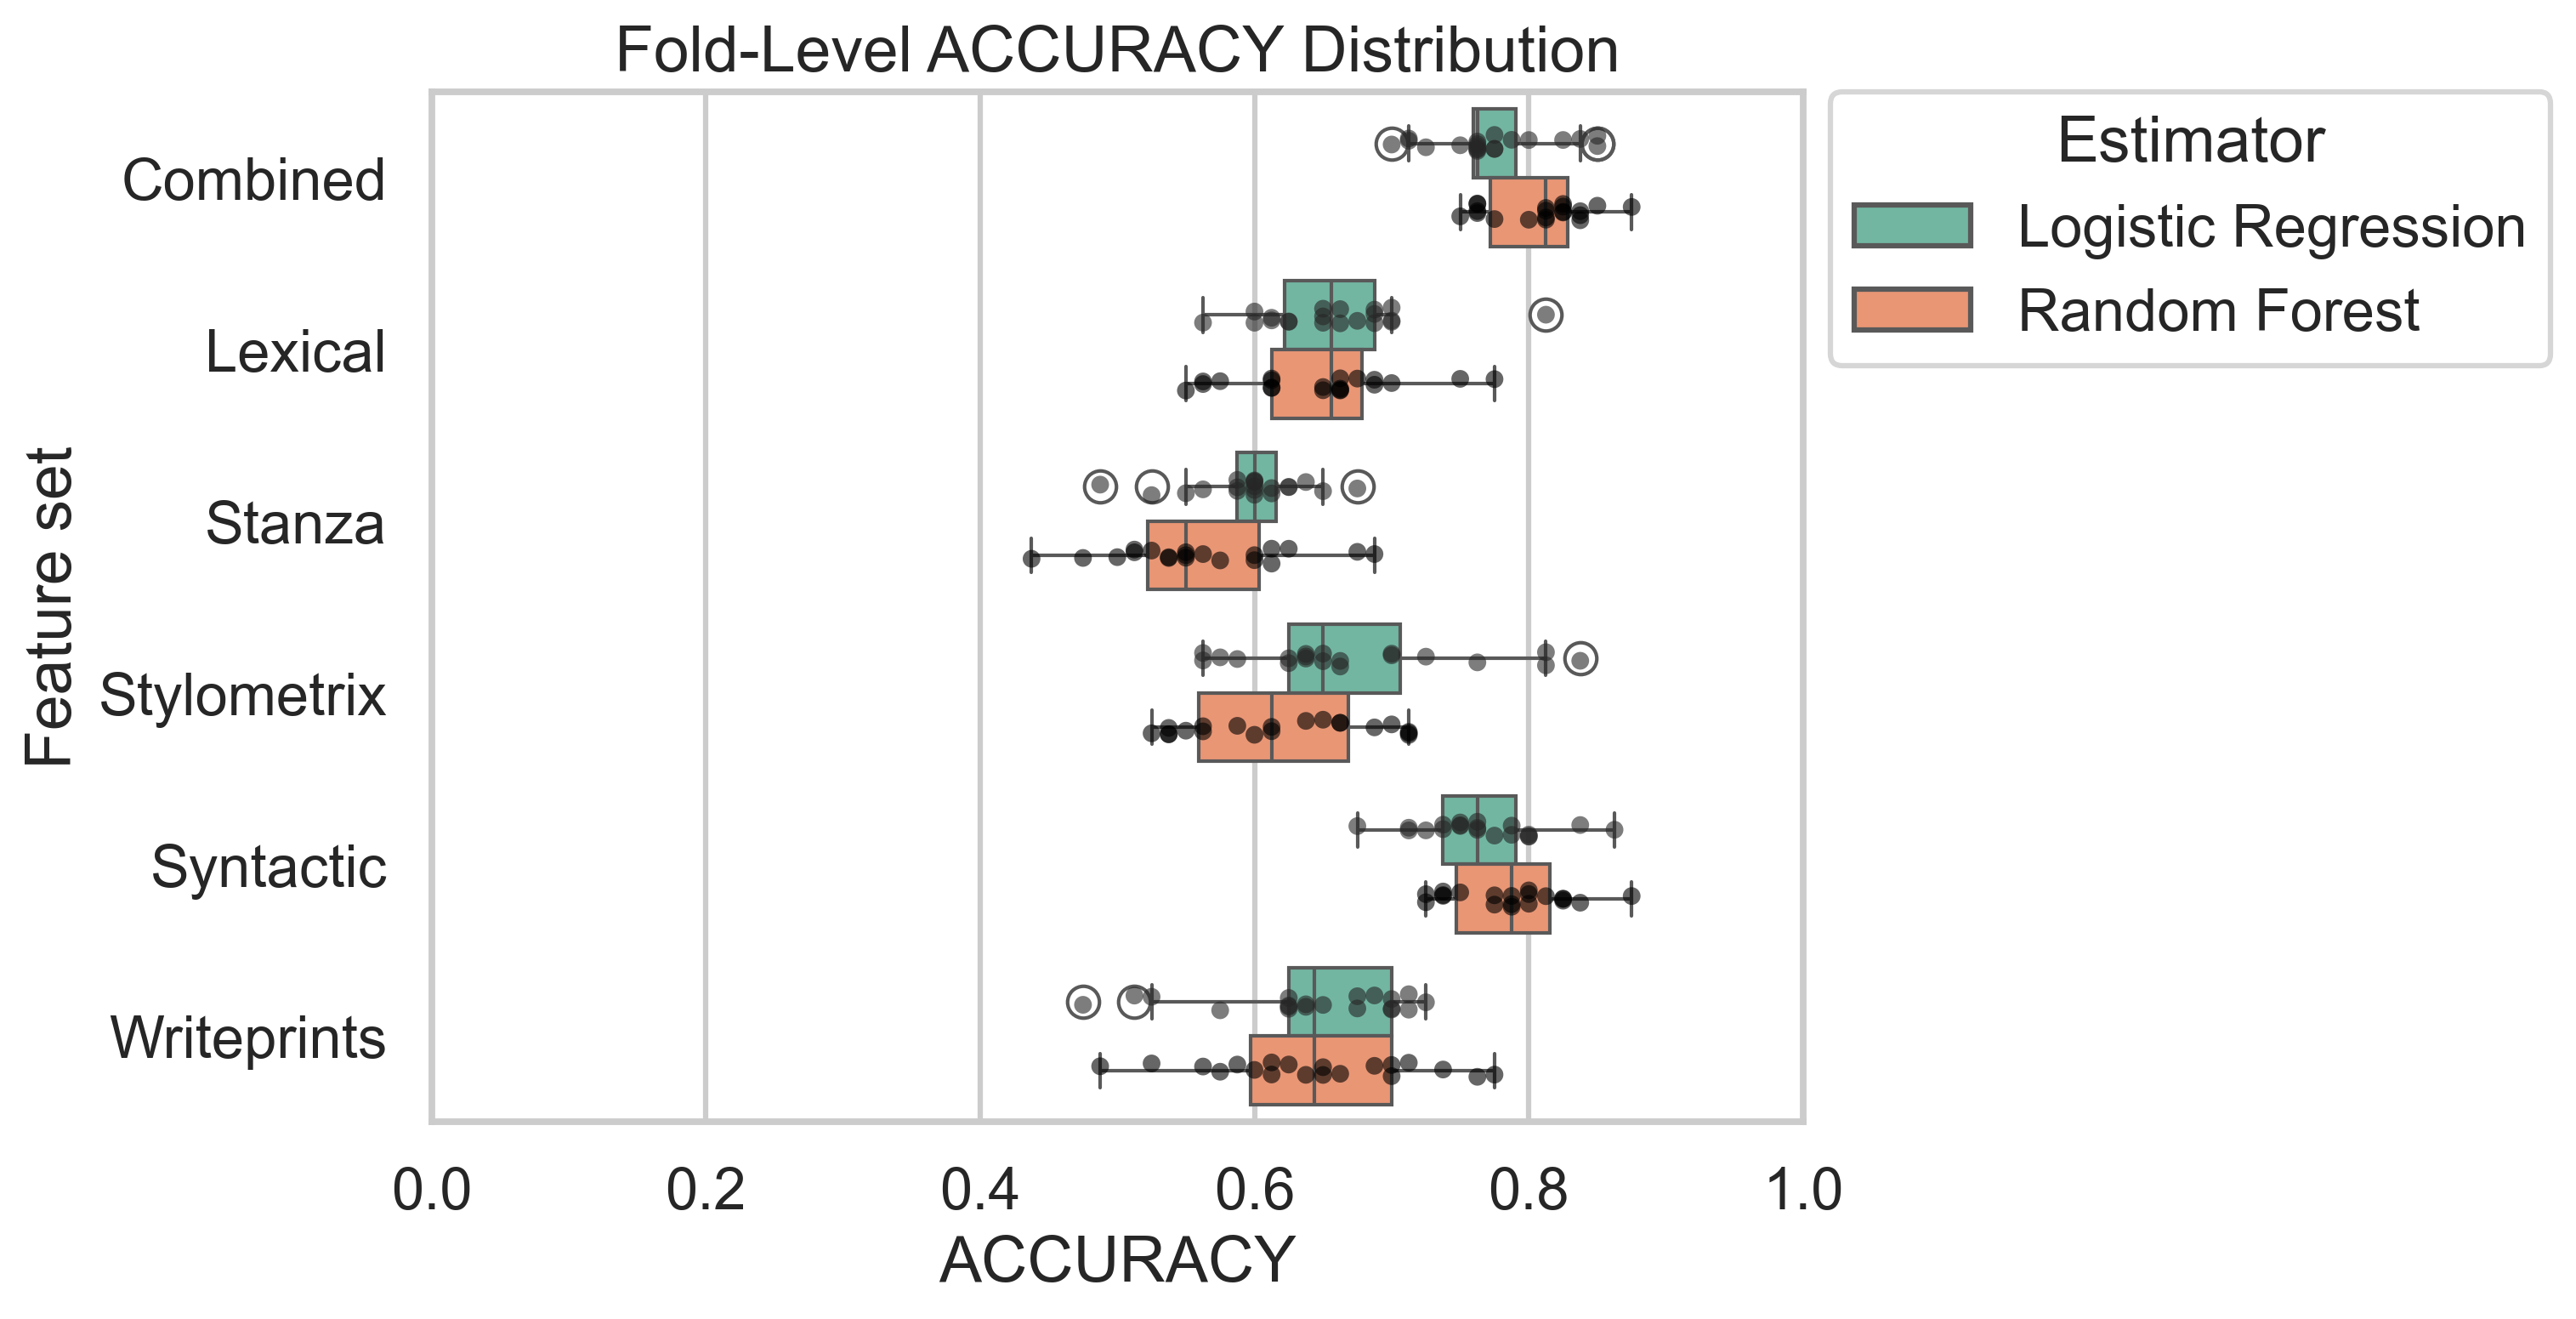
\includegraphics[width=0.9\textwidth]{results/v2/figures/accuracy_fold_distribution.png}
\caption{Supplementary fold-level binary accuracy distribution across feature sets and estimators.}
\label{fig:appendix-accuracy-folds}
\end{figure}

\begin{figure}[H]
\centering
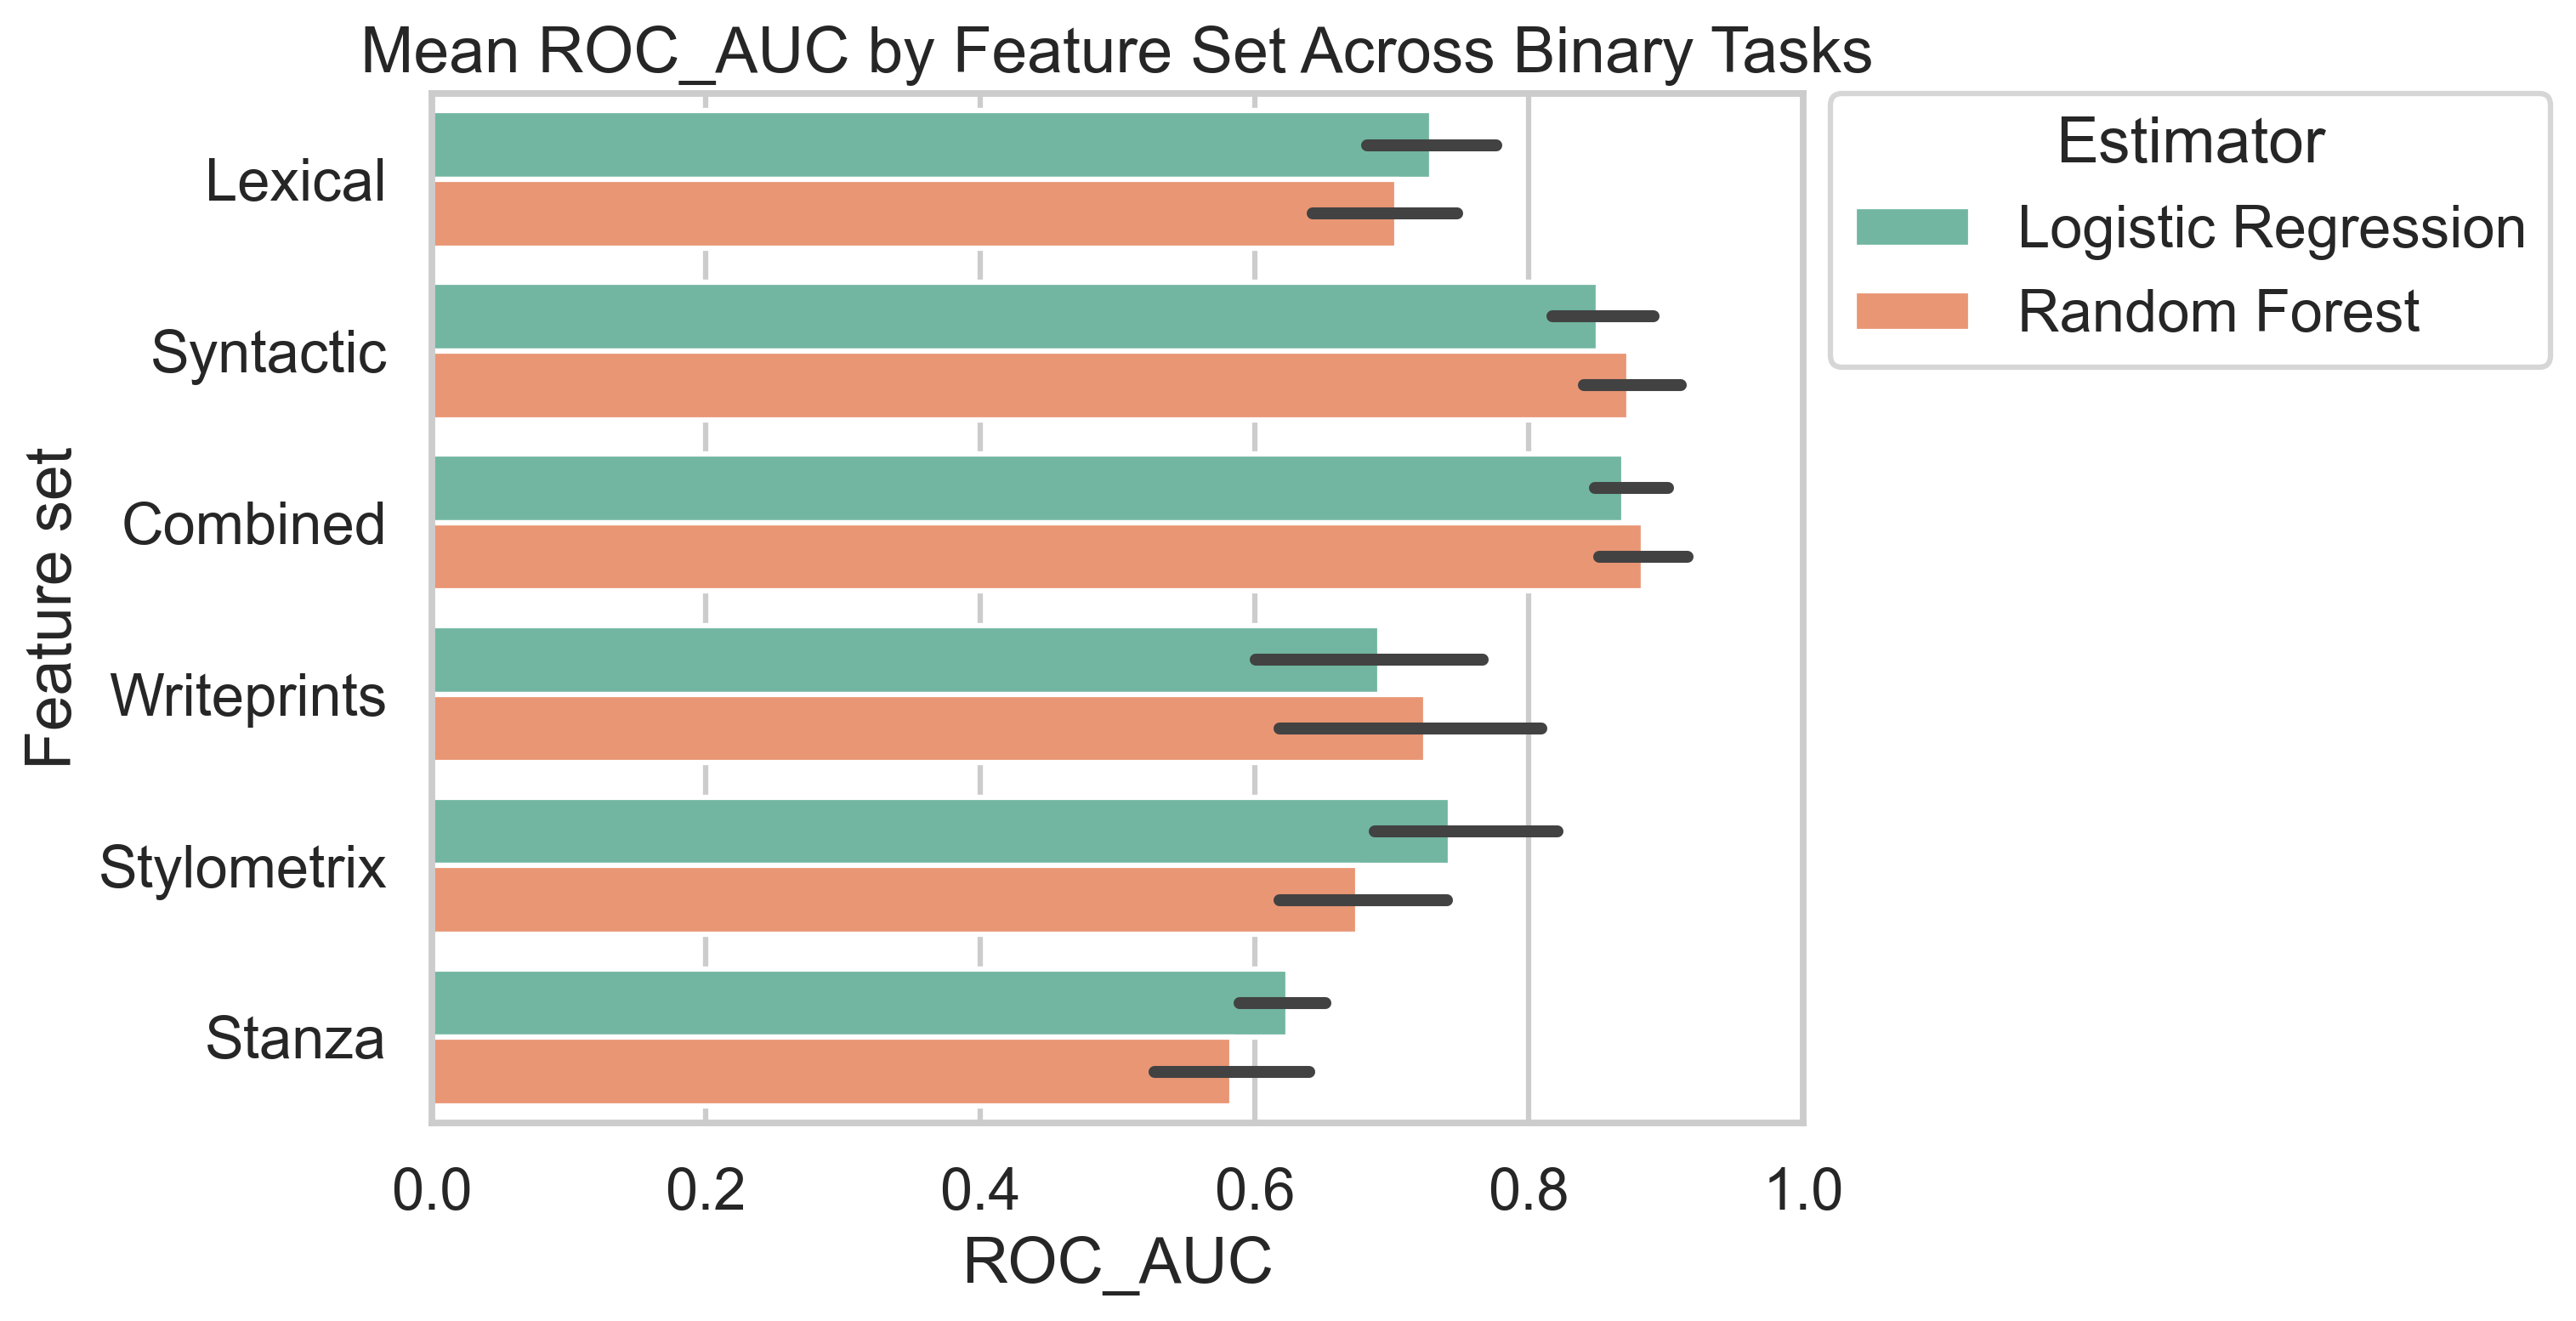
\includegraphics[width=0.9\textwidth]{results/v2/figures/roc_auc_by_feature_set.png}
\caption{Supplementary binary ROC-AUC by feature set and estimator, showing separability across thresholds rather than only hard-label performance.}
\label{fig:appendix-roc-feature}
\end{figure}

\begin{figure}[H]
\centering
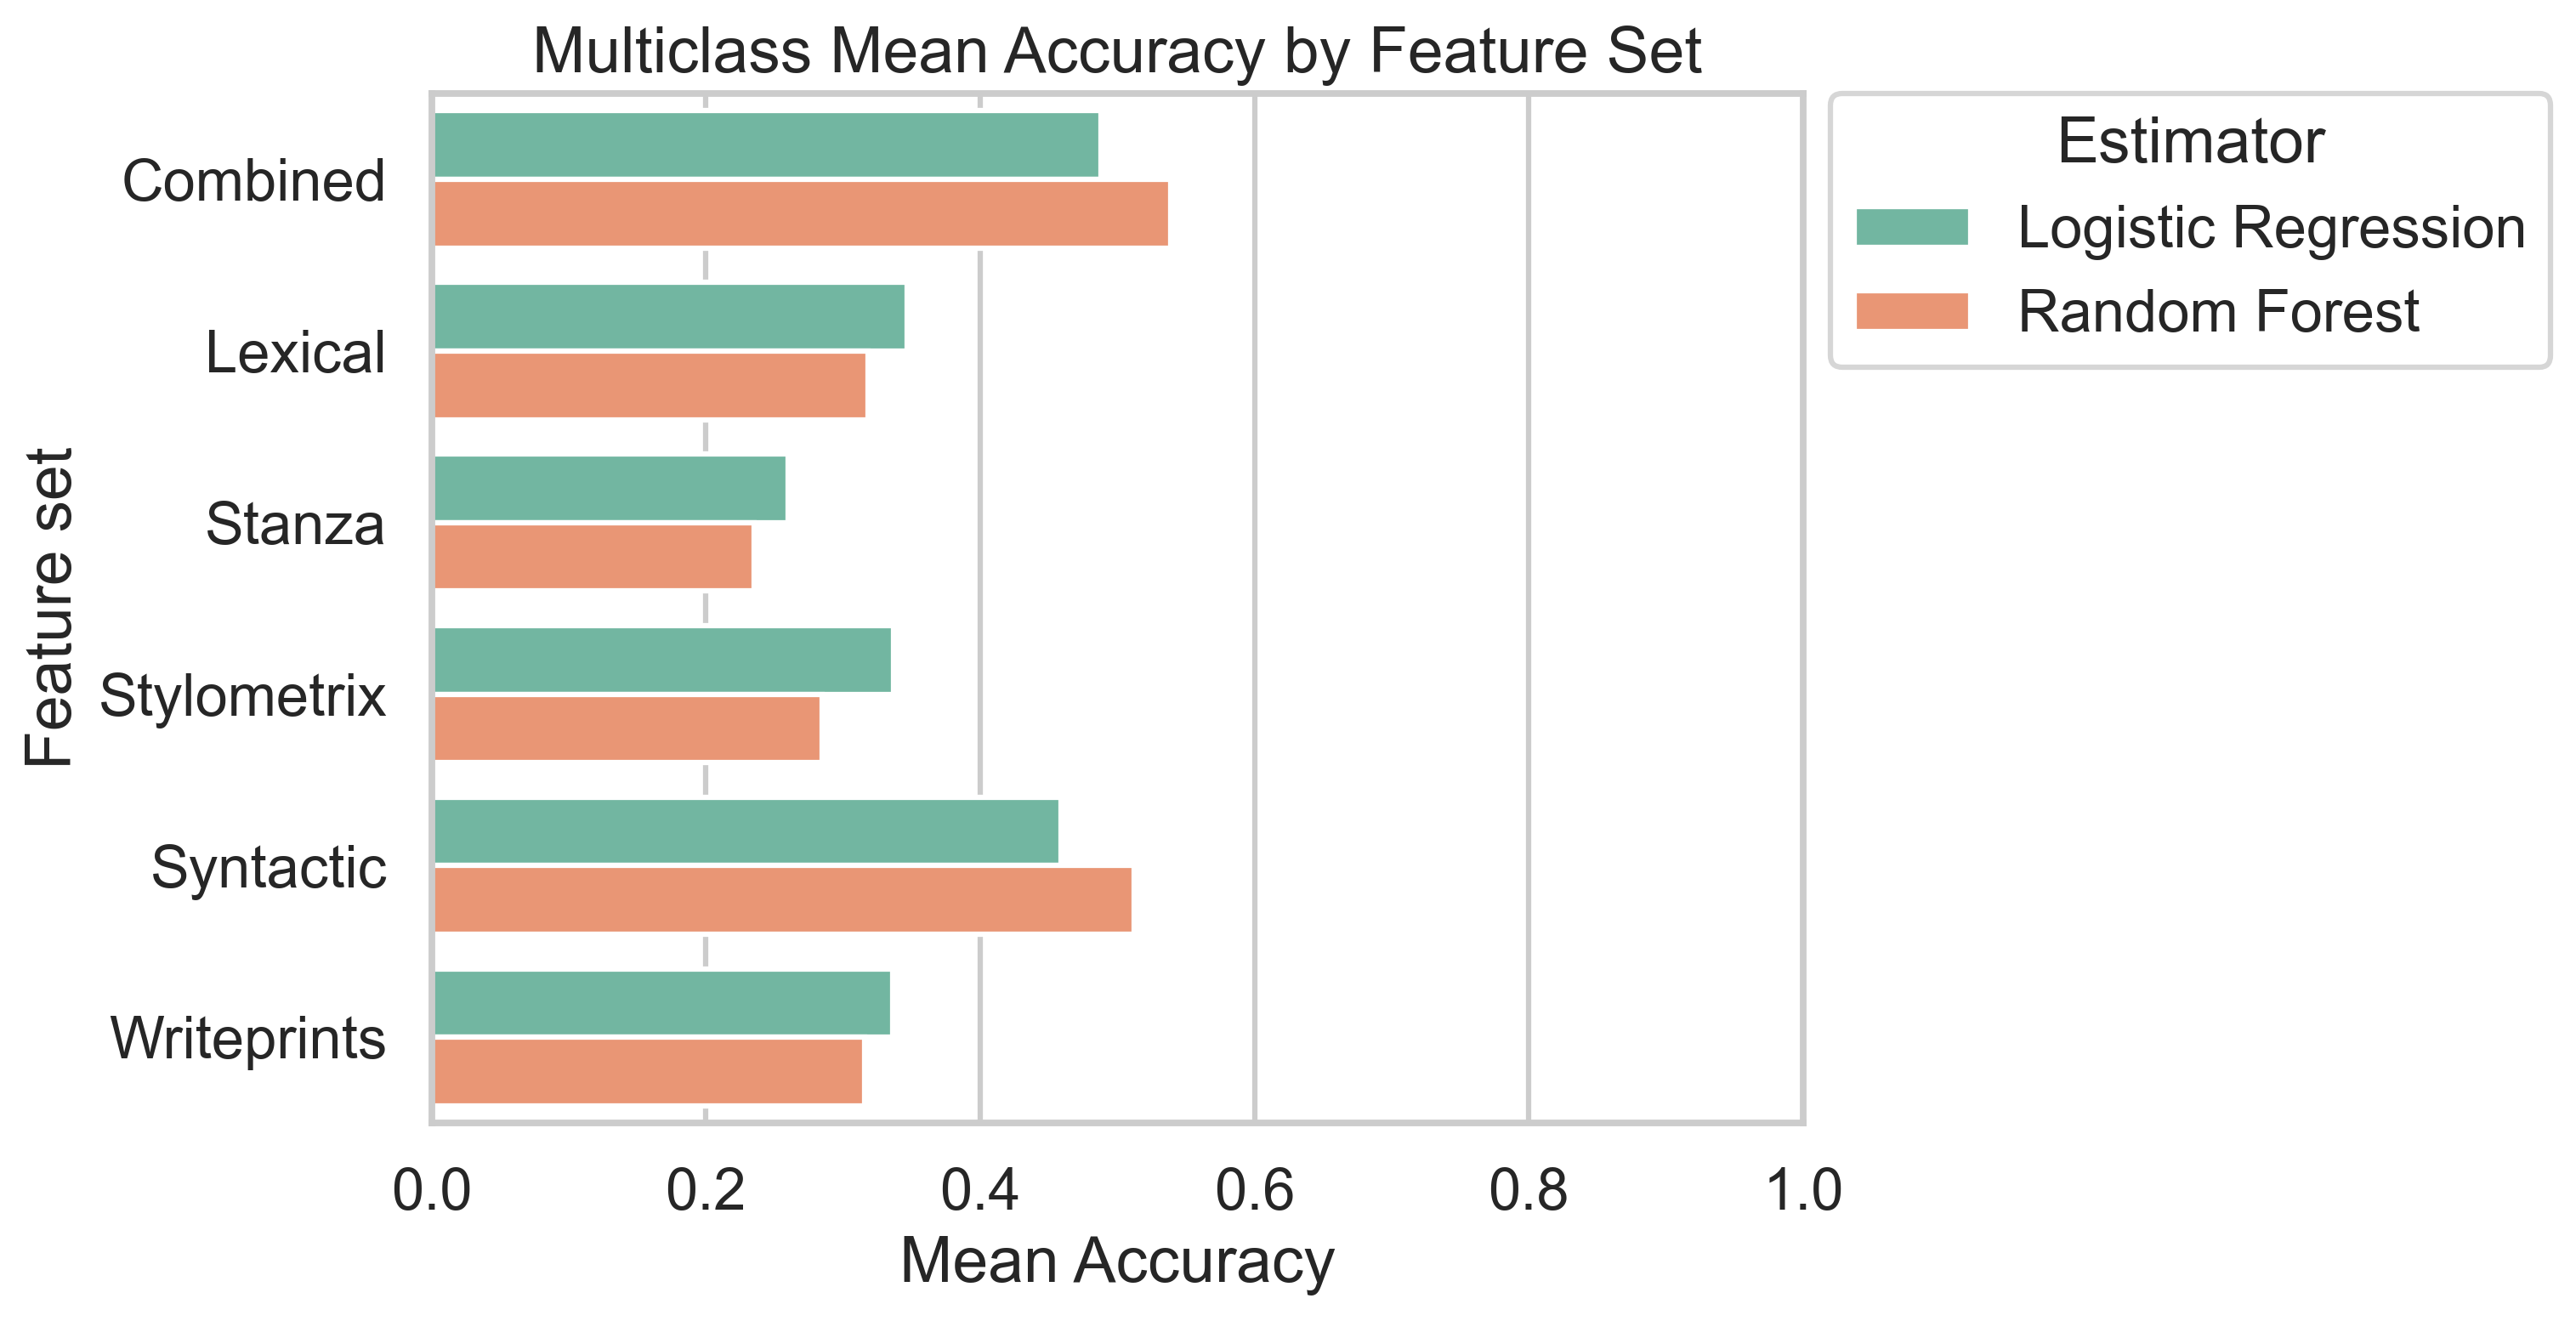
\includegraphics[width=0.9\textwidth]{results/v2/figures/multiclass_accuracy_mean.png}
\caption{Supplementary multiclass mean accuracy by feature set and estimator. This supports the multiclass macro-F1 figure in the main report.}
\label{fig:appendix-multiclass-accuracy}
\end{figure}

\begin{figure}[H]
\centering
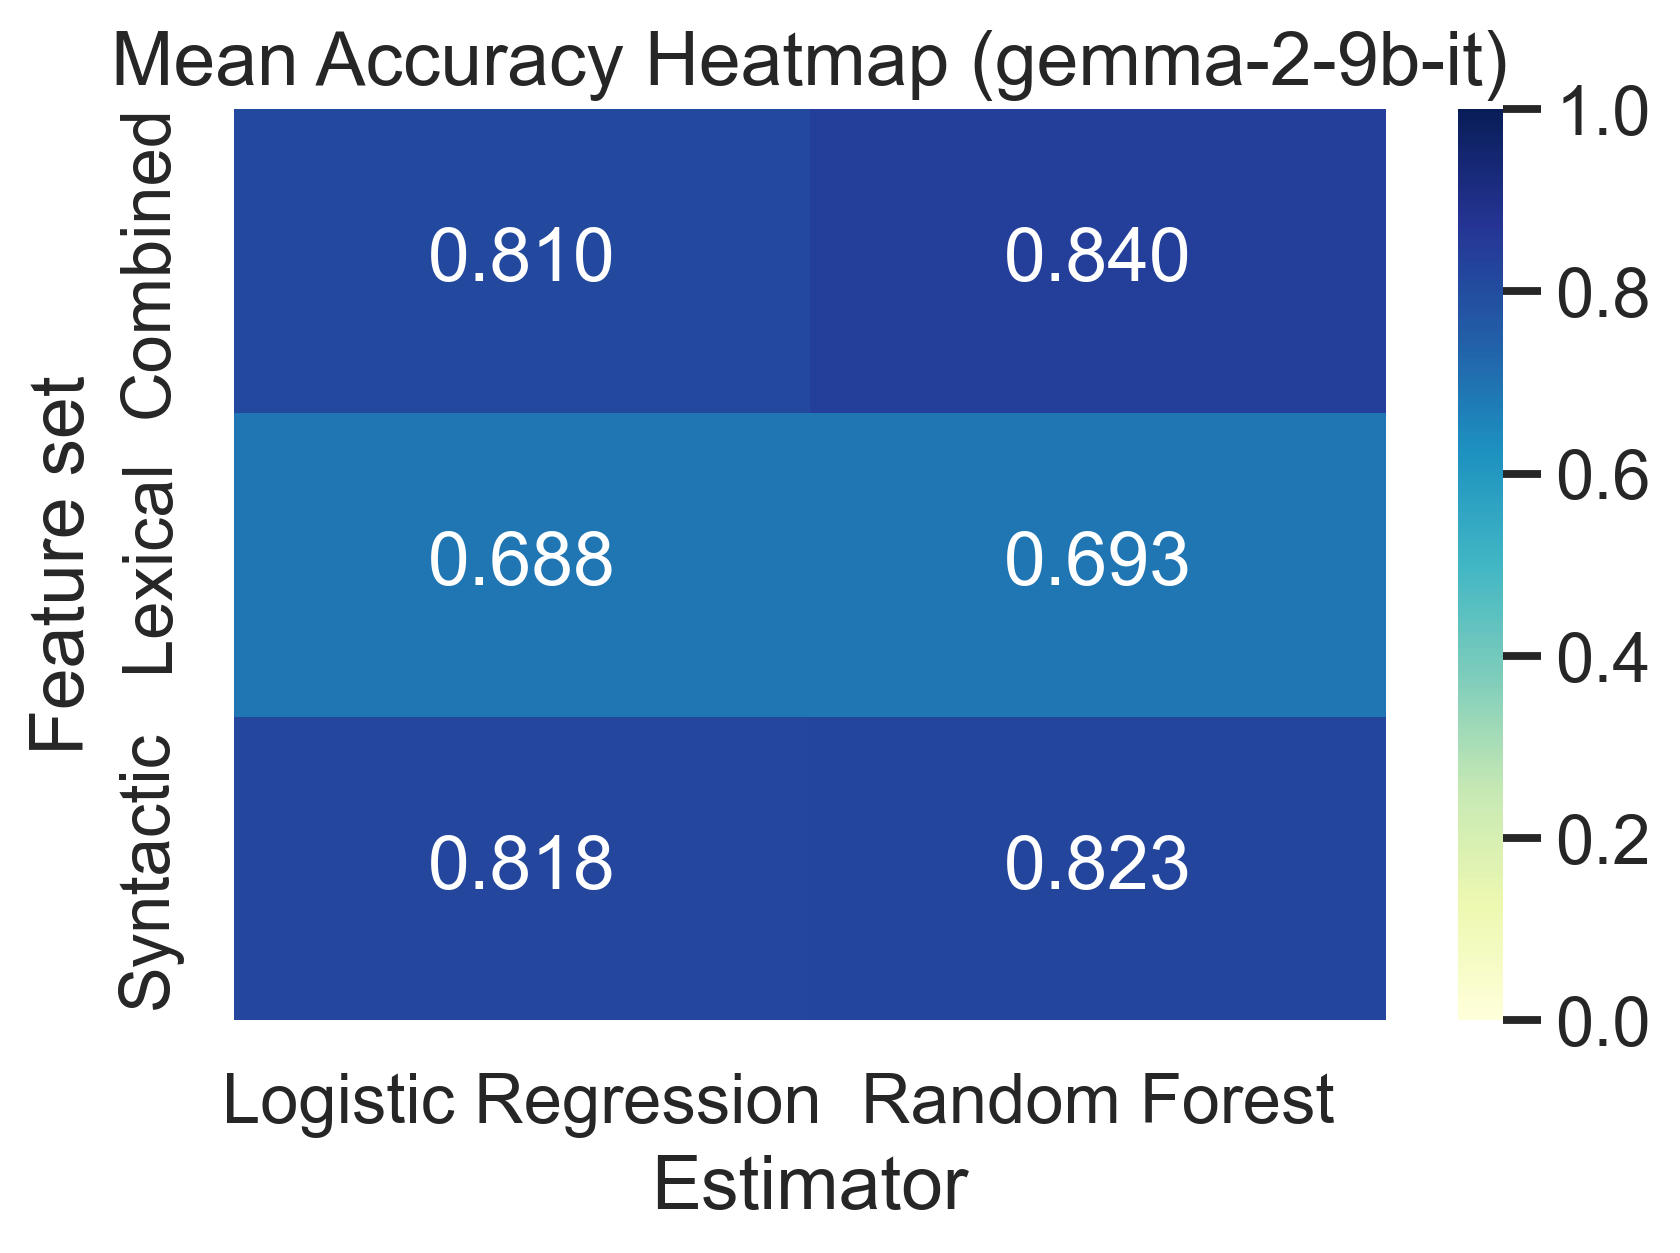
\includegraphics[width=0.9\textwidth]{results/v2/figures/gemma-2-9b-it_accuracy_heatmap.png}
\caption{Supplementary Gemma binary accuracy heatmap across feature sets and estimators.}
\label{fig:appendix-gemma-heatmap}
\end{figure}

\subsubsection{Supplementary Tables}

\begin{table}[H]
\centering
\small
\begin{tabular}{llrrr}
\toprule
Feature set & Estimator & Accuracy & Macro-F1 & ROC-AUC \\
\midrule
lexical & Logistic Regression & 0.347 & 0.333 & 0.680 \\
lexical & Random Forest & 0.318 & 0.316 & 0.633 \\
syntactic & Logistic Regression & 0.459 & 0.454 & 0.776 \\
syntactic & Random Forest & 0.512 & 0.504 & 0.804 \\
combined & Logistic Regression & 0.488 & 0.484 & 0.803 \\
combined & Random Forest & 0.539 & 0.538 & 0.821 \\
writeprints & Logistic Regression & 0.336 & 0.328 & 0.663 \\
writeprints & Random Forest & 0.316 & 0.310 & 0.660 \\
stylometrix & Logistic Regression & 0.337 & 0.311 & 0.667 \\
stylometrix & Random Forest & 0.285 & 0.282 & 0.594 \\
stanza & Logistic Regression & 0.260 & 0.244 & 0.583 \\
stanza & Random Forest & 0.235 & 0.233 & 0.541 \\
\bottomrule
\end{tabular}
\caption{Full multiclass summary by feature family and estimator. This table supports the main multiclass discussion while keeping the body of the report focused on the strongest results.}
\label{tab:appendix-multiclass-full}
\end{table}

\begin{table}[H]
\centering
\small
\begin{tabular}{lrrrrr}
\toprule
Classifier & Accuracy & Precision & Recall & F1 & ROC-AUC \\
\midrule
Logistic Regression & 0.750 & 0.793 & 0.676 & 0.730 & 0.891 \\
Random Forest & 0.824 & 0.893 & 0.735 & 0.806 & 0.898 \\
\bottomrule
\end{tabular}
\caption{Additional factual-prompt baseline metrics retained as supporting evidence. These outputs are not part of the main v2 comparison.}
\label{tab:appendix-factual-metrics}
\end{table}

\begin{table}[H]
\centering
\small
\begin{tabular}{lrr}
\toprule
Actual class & Predicted human & Predicted LLM \\
\midrule
human & 31 & 3 \\
LLM & 9 & 25 \\
\bottomrule
\end{tabular}
\caption{Confusion matrix for the saved factual-prompt baseline model. This provides a compact error profile for the supporting baseline run.}
\label{tab:appendix-factual-confusion}
\end{table}

\begin{table}[H]
\centering
\small
\begin{tabular}{lr}
\toprule
Feature & Mean absolute SHAP value \\
\midrule
\texttt{avg\_sentence\_len\_words} & 0.055 \\
\texttt{std\_sentence\_len\_words} & 0.050 \\
\texttt{avg\_word\_len} & 0.035 \\
\texttt{fw\_of\_per100w} & 0.029 \\
\texttt{punct\_41\_per100w} & 0.025 \\
\texttt{fw\_this\_per100w} & 0.025 \\
\texttt{type\_token\_ratio} & 0.024 \\
\texttt{fw\_to\_per100w} & 0.023 \\
\texttt{sentence\_count} & 0.020 \\
\texttt{punct\_40\_per100w} & 0.020 \\
\bottomrule
\end{tabular}
\caption{Top ten SHAP features from the supporting factual baseline. The strongest values are mainly sentence-length, word-length, function-word, and punctuation features, which is consistent with the report's emphasis on structural stylistic evidence.}
\label{tab:appendix-shap-top}
\end{table}

\begin{table}[H]
\centering
\small
\begin{tabularx}{\textwidth}{lX}
\toprule
Saved file & Purpose \\
\midrule
\texttt{master\_with\_features.csv} & Combined human and generated corpus with extracted feature columns. \\
\texttt{summary\_binary.csv} & Cross-validated binary results for each target model, feature family, and estimator. \\
\texttt{summary\_multiclass.csv} & Cross-validated five-class attribution results. \\
\texttt{semantic\_pair\_scores.csv} & Source-level semantic-overlap scores between human abstracts and generated rewrites. \\
\texttt{binary\_metric\_summary.csv} & Plot-ready summary of binary accuracy, F1, ROC-AUC, and MCC. \\
\texttt{run\_manifest.json} & Record of the analysis run settings and generated outputs. \\
\bottomrule
\end{tabularx}
\caption{Key supplementary result files retained for reproducibility and auditability.}
\label{tab:appendix-output-files}
\end{table}

\end{document}
